%%%%%%%%%%%%%%%%%%%%%%% file template.tex %%%%%%%%%%%%%%%%%%%%%%%%%
%
% This is a general template file for the LaTeX package SVJour3
% for Springer journals.          Springer Heidelberg 2010/09/16
%
% Copy it to a new file with a new name and use it as the basis
% for your article. Delete % signs as needed.
%
% This template includes a few options for different layouts and
% content for various journals. Please consult a previous issue of
% your journal as needed.
%
%%%%%%%%%%%%%%%%%%%%%%%%%%%%%%%%%%%%%%%%%%%%%%%%%%%%%%%%%%%%%%%%%%%
%
% First comes an example EPS file -- just ignore it and
% proceed on the \documentclass line
% your LaTeX will extract the file if required
\begin{filecontents*}{example.eps}
%!PS-Adobe-3.0 EPSF-3.0
%%BoundingBox: 19 19 221 221
%%CreationDate: Mon Sep 29 1997
%%Creator: programmed by hand (JK)
%%EndComments
gsave
newpath
  20 20 moveto
  20 220 lineto
  220 220 lineto
  220 20 lineto
closepath
2 setlinewidth
gsave
  .4 setgray fill
grestore
stroke
grestore
\end{filecontents*}
%
\RequirePackage{fix-cm}
%
%\documentclass{svjour3}                     % onecolumn (standard format)
%\documentclass[smallcondensed]{svjour3}     % onecolumn (ditto)
\documentclass[smallextended]{svjour3}       % onecolumn (second format)
%\documentclass[twocolumn]{svjour3}          % twocolumn
%
\smartqed  % flush right qed marks, e.g. at end of proof
%
\usepackage{amsmath}
\usepackage{xspace,stmaryrd,latexsym,url}
\usepackage{graphicx,tikz,rotating}
\usepackage[strings]{underscore}

\usepackage{cite}

%\usepackage{authblk}

%
% \usepackage{mathptmx}      % use Times fonts if available on your TeX system
%
% insert here the call for the packages your document requires
%\usepackage{latexsym}
% etc.
%
% please place your own definitions here and don't use \def but
% \newcommand{}{}
%
% Insert the name of "your journal" with
% \journalname{myjournal}
%


\def\D{\mathit{D}}
\def\E{\mathit{E}}

\def\FFOL{\entity{FFOL}\xspace}
\def\V{\mathit{V}}
\def\F{\mathit{F}}
\def\P{\mathit{P}}
\def\True{\mathit{True}}
\def\False{\mathit{False}}
\def\Impl{\rightarrow}
\def\Descr{\rotatebox[origin=C]{180}{$\iota$}}
%\def\Descr{\rotate[c]{180}{\iota}}


% -----------------------------------------------

\def\lambdot{\rule{0.6mm}{0.6mm}\hspace{0.4ex}} 
\def\all#1{\forall #1\lambdot}
\def\exi#1{\exists #1\lambdot}
\def\lam#1{\lambda #1\lambdot}


\def\modal#1{#1}
\def\mfalse{\modal\bot}
\def\mtrue{\modal\top}
\def\mnot{\modal\neg\,}
\def\mor{\,\modal\vee\,}
\def\mand{\,\modal\wedge\,}
\def\mimpl{\,\modal\supset\,}
\def\miff{\,\modal\Leftrightarrow\,}
\def\mball#1{\modal\Box_{#1}\,}
\def\mdexi#1{\modal\Diamond_{#1}\,}
\def\mall#1{\modal{\forall}{#1}\lambdot\,}
\def\mexi#1{\modal{\exists}{#1}\lambdot\,}
\def\mpi{\modal{\Pi}\,}
\def\mvalid{\modal{\texttt{valid}}} 

\def\Metaeq{=}
\def\bnormform#1{\left.#1\hspace*{-.4ex}\right\downarrow_\beta}
\def\benormform#1{\left.#1\hspace*{-.4ex}\right\downarrow_{\beta\eta}}
\def\Bnormform#1{\left.{#1}\hspace*{-.4ex}\right\downarrow_\beta}
\def\Benormform#1{\left.{#1}\hspace*{-.4ex}\right\downarrow_{\beta\eta}}
\def\ambnormform#1{{#1}\hspace*{-1.1ex}\downarrow_{\kern-.2em\scriptscriptstyle *}} % ``ambiguous'' normal form
\def\eqb{\Metaeq_{\beta}}
\def\eqe{\Metaeq_{\eta}}
\def\eqbe{\Metaeq_{\beta\eta}}
\def\convarrow{\rightarrow}


\newcommand\entity[1]{\text{\textrm{#1}}}
\def\QHL{\entity{QHL}}
\def\QML{\entity{QML}}
\def\NOM{\entity{NOM}}
\def\SVAR{\entity{SVAR}}
\def\CON{\entity{CON}}
\def\FVAR{\entity{FVAR}}
%\def\IC{\entity{IC}}
\def\FSYM{\entity{FSYM}}
\def\RSYM{\entity{RSYM}}
\def\QHLSTT{\entity{QHLSTT}}
\def\QMLSTT{\entity{QMLSTT}}
\def\IV{\entity{IV}}
\def\PV{\entity{PV}}
\def\SYM{\entity{SYM}}
\def\IVSTT{\entity{IVSTT}}
\def\PVSTT{\entity{PVSTT}}
\def\SYMSTT{\entity{SYMSTT}}
\def\SSTT{\entity{SSTT}}
\def\AR{\entity{AR}}
\def\STT{\entity{STT}\xspace}

\def\QKPIm{\entity{QK}\pi^-\xspace}
\def\QKPI{\entity{QK}\pi\xspace}
\def\QKPIp{\entity{QK}\pi^+\xspace}
\def\QSFPIm{\entity{QS5}\pi^-\xspace}
\def\QSFPI{\entity{QS5}\pi\xspace}
\def\QSFPIp{\entity{QS5}\pi^+\xspace}

\def\stt{\entity{STT}\xspace}
\def\tt{\entity{STT}}
\def\lm{\entity{MM}\xspace}
\def\ipl{\entity{IPL}\xspace}
\def\HOML{\entity{HOML}\xspace}
\def\HOL{\entity{HOL}\xspace}

\def\worldtype{\mu}
\def\indtype{\iota}
\def\mutype{\mu}
\def\boola{\omicron}
\def\boolb{\hat{\omicron}}

\def\ar{\shortrightarrow}

\newcommand\map[1]{\widehat{#1}}
\newcommand\hol[1]{\boldsymbol{#1}}
\newcommand\lift[1]{\lceil #1 \rceil}
\newcommand\llift[1]{\dot{#1}}

\newcommand{\imp}{\longrightarrow}
\newcommand{\limp}{\longleftarrow}
\newcommand{\biimp}{\longleftrightarrow}
\newcommand{\allq}{\forall}
\newcommand{\exq}{\exists}
\newcommand{\seq}{\vdash}
\newcommand{\nec}{\Box} % necessarily
\newcommand{\pos}{\Diamond} % possibly
\newcommand{\ess}[2]{#1 \ \mathit{ess.} \ #2}
\newcommand{\NE}{\mathit{NE}}


\def\ti{i}
\def\dom{\textit{dom \/}}
\def\cod{\textit{cod \/}}
\def\comp{\cdot}
\def\kleq{\cong}
\def\exid{\simeq}
\def\ddef{:=}
\def\id{\textit{I\/}}
\def\ex{\E}


\newtheorem{thm}{Theorem} 
\newtheorem{defn}[thm]{Definition}
\newtheorem{lem}[thm]{Lemma}



\begin{document}

\title{Automating Free Logic in HOL, with an Experimental Application in Category Theory}
%\title{Free Logic and Axiom Systems for Category Theory in HOL\thanks{Mention DFG grants ...}}
%\title{Embedding Free Logic and Axiom Systems for Category Theory in HOL\thanks{Mention DFG grants ...}}
%\subtitle{(And an Exemplary Application in Category Theory)}

\titlerunning{Automating Free Logic in HOL}        % if too long for running head


\author{Christoph Benzm\"uller\thanks{Benzmüller received funding from the German National Research
  Foundation DFG under Heisenberg grant \emph{Towards Computational
    Metaphysics} (BE 2501/9-2) and from VolkswagenStiftung under grant
  Consistent Rational Argumentation in Politics (CRAP).}  and Dana S. Scott}
\institute{Christoph Benzm\"uller \at
   Freie Universit\"at Berlin, Berlin, Germany \& University of Luxembourg, Luxembourg\\
%   Stanford University, CSLI/Cordura Hall, Stanford, CA 94305-4115, U.S. \\
   \email{c.benzmueller@gmail.com} \\
% \\
 %            \emph{Present address:} of F. Author  %  if needed
Dana S. Scott \at
Visiting Scholar at University of California, Berkeley,  USA \\
  \email{dana.scott@cs.cmu.edu}
}

\date{\today}                     %% if you don't need date to appear

% \author{Christoph Benzm\"uller       \and
%       Dana Scott 
% }

%\authorrunning{Short form of author list} % if too long for running head

% \institute{F. Author \at
%               first address \\
%               Tel.: +123-45-678910\\
%               Fax: +123-45-678910\\
%               \email{fauthor@example.com}           %  \\
% %             \emph{Present address:} of F. Author  %  if needed
%            \and
%            S. Author \at
%               second address
% }

\date{Received: date / Accepted: date}
% The correct dates will be entered by the editor


\maketitle

\begin{abstract}
  % Partiality and undefinedness are prominent challenges in various
  % areas of mathematics and computer science.  Unfortunately, however,
  % modern proof assistant system based on traditional classical or
  % intuitionistic logics provide rather inadequate support for these
  % challenge concepts.  Free logic offers a theoretically appealing
  % solution, but is has been considered as rather unsuited towards
  % practical utilisation.

  % The two main contributions of this article are: (i) A shallow
  % semantical embedding of free logic in classical higher-order logic
  % is presented; this embedding enables the application of higher-order
  % interactive and automated theorem provers (and their integrated
  % subprovers) for the formalisation and verification of free logic
  % theories.  (ii) This approach to automate free logic is exemplarily
  % employed in a selected domain of mathematics: Starting from a
  % generalization of the standard axioms for a monoid we present a
  % stepwise development of various, mutually equivalent foundational
  % axiom systems for category theory. As a side-effect of this work
  % some (minor) issue in a prominent category theory textbook have been
  % revealed.

  A shallow semantical embedding of free logic in classical
  higher-order logic is presented, which enables the off-the-shelf
  application of higher-order interactive and automated theorem
  provers for the formalisation and
  verification of free logic theories.  
  Subsequently, this approach is applied to a selected domain of
  mathematics:
 starting from a generalization of the standard axioms
  for a monoid we present a stepwise development of various, mutually
  equivalent foundational axiom systems for category theory. As a
  side-effect of this work some (minor) issues in a prominent category
  theory textbook have been revealed.

  The purpose of this article is not to claim any novel results in
  category theory, but to demonstrate an elegant way to ``implement''
  and utilize interactive and automated reasoning in free logic, and
  to present illustrative experiments.


\keywords{Free Logic \and Classical Higher-Order Logic \and Category
  Theory \and Interactive and Automated Theorem Proving }
% \PACS{PACS code1 \and PACS code2 \and more}
% \subclass{MSC code1 \and MSC code2 \and more}
\end{abstract}

\section{Introduction}
\label{intro}
Partiality and undefinedness are prominent challenges in various areas
of mathematics and computer science.  Unfortunately, however, modern
proof assistant systems and automated theorem provers based on
traditional classical or intuitionistic logics provide rather
inadequate support for these challenge concepts.  Free logic \cite{Lambert60,Scott67,lambert02:_free_logic,sep-logic-free} offers a
theoretically appealing solution, but it has been considered as rather
unsuited towards practical utilization.


In the first part of this article (\S2 and \S3) we show how free logic
can be elegantly ``implemented'' in any theorem proving system for
classical higher-order logic (HOL) \cite{B5}. The proposed solution
employs a semantic embedding of free logic in HOL. We present, as an
example, one implementation of this idea in the proof
assistant Isabelle/HOL \cite{NPW02}. Various state-of-the-art
first-order and higher-order automated theorem provers and model
finders are integrated (modulo suitable logic translations) with
Isabelle via the Sledgehammer tool \cite{Sledgehammer}, so that our
solution can be utilized, via Isabelle as foreground system, with a
whole range of other background reasoners, such as SMT solvers and
first-order and higher-order automated theorem
provers.\footnote{Cf.~\S\ref{sec-remarks-experiments} for further
  information.} As a result we obtain an
elegant and powerful implementation of an interactive and automated
theorem proving (and model finding) system for free logic.


%   The two main contributions of this article are: (i) A shallow
%   semantical embedding of free logic in classical higher-order logic
%   is presented; this embedding enables the application of higher-order
%   interactive and automated theorem provers (and their integrated
%   subprovers) for the formalisation and verification of free logic
%   theories.  (ii) This approach to automate free logic is exemplarily
%   employed in a selected domain of mathematics: Starting from a
%   generalization of the standard axioms for a monoid we present a
%   stepwise development of various, mutually equivalent foundational
%   axiom systems for category theory. As a side-effect of this work
%   some (minor) issue in a prominent category theory textbook have been
%   revealed.



% Partiality and undefinedness are core concepts in various areas of
% mathematics.  Modern mathematical proof assistants and theorem proving
% systems are often based on traditional classical or intuitionistic
% logics and provide rather inadequate support for these challenge
% concepts.  Free logic @{cite "sep-logic-free,scott67:exist"}, in
% contrast, offers a theoretically and practically appealing
% solution. Unfortunately, however, we are not aware of any implemented
% and available theorem proving system for free logic.
 
% In this extended abstract we show how free logic can be
% ``implemented'' in any theorem proving system for classical
% higher-order logic (HOL) @{cite "B5"}. The proposed solution employs a
% semantic embedding of free (or inclusive logic) in HOL. We present an
% exemplary implementation of this idea in the mathematical proof
% assistant Isabelle/HOL @{cite "NPW02"}. Various state-of-the-art
% first-order and higher-order automated theorem provers and model
% finders are integrated (modulo suitable logic translations) with
% Isabelle via the Sledgehammer tool @{cite "Sledgehammer"}, so that our
% solution can be utilized, via Isabelle as foreground system, with a
% whole range of other background reasoners. As a result we obtain an
% elegant and powerful implementation of an interactive and automated
% theorem proving (and model finding) system for free logic.
  
To demonstrate the practical relevance of our new system, we present
in \S4 a stepwise development of axioms
systems for category theory by generalizing the standard axioms for a
monoid to a partial composition operation. Our purpose is not to make
or claim any contribution to category theory but rather to show how
formalizations involving the kind of logic required (free logic) can
be implemented and validated within modern proof assistants such as
Isabelle/HOL.  We also address the relation of our axiom systems to
alternative proposals from the literature, including an axiom set
proposed by Freyd and Scedrov in their textbook ``Categories,
Allegories'' \cite{FreydScedrov90} for which we reveal a technical
flaw: either all operations, e.g. morphism composition, are total or
their axiom system is inconsistent. The repair for this problem is
quite straightforward, however. The solution essentially corresponds
to a set of axioms proposed by Scott \cite{Scott79} in the 1970s.

% \marginpar{will rewrite this part}
% A total of eight different axiom systems is studied. The systems I-VI
% are shown to be equivalent. The axiom system VII slightly modifies
% axiom system VI to obtain (modulo notational transformation) the set
% of axioms as proposed by Freyd and Scedrov in their textbook
% ``Categories, Allegories'' \cite{FreydScedrov90}, published in 1990;
% see also Subsection \ref{subsec:FreydNotation} where we present their
% original system.  While the axiom systems I-VI are shown to be
% consistent, a constricted inconsistency result is obtained for system
% VII (when encoded in free logic where free variables range over all
% objects): We can prove $\exists x\lambdot \neg(\ex x) \Impl False$, where
% $\ex$ is the existence predicate. Read this as: If there are undefined
% objects, e.g. the value of an undefined composition $x\cdot y$
% then we have falsity.  By contraposition, all objects (and thus all
% compositions) must exist. But when we assume the latter, then the
% axiom system VII essentially reduces categories to monoids.  We note
% that axiom system V, which avoids this problem, corresponds to a set
% of axioms proposed by Scott \cite{Scott79} in the 1970s. The
% problem can also be avoided by restricting the variables in axiom
% system VII to range only over existing objects and by postulating
% strictness conditions.  This gives us axiom system VIII.

Our exploration has been significantly supported by series of
experiments in which automated reasoning tools have been called from
within the proof assistant Isabelle/HOL via the
Sledgehammer tool. Moreover, we have obtained
very useful feedback at various stages from the model finder Nitpick
\cite{Nitpick}, saving us from making several mistakes.

At the conceptual level this paper exemplifies a new style of
explorative mathematics which rests on a significant amount of
human-machine interaction with integrated interactive-auto\-ma\-ted
theorem proving technology. The experiments we have conducted are such
that the required reasoning is often too tedious and time-consuming
for humans to be carried out repeatedly with highest level of
precision. It is here where cycles of formalization and
experimentation efforts in Isabelle/HOL provided significant
support. Moreover, the technical inconsistency issue for axiom system
VII was discovered by automated theorem provers, which further
emphasizes the added value of automated theorem proving in this area.

The content of article is based on the 
contributions reported in two previous papers \cite{ICMS,ArXiv}.

% To enable our experiments we have exploited an embedding of free logic @{cite "Scott67"} 
% in classical higher-order logic, which we have recently presented in a related paper @{cite "C57"}.


% We also want to emphasize that this paper has been written entirely within the Isabelle 
% framework by utilizing the Isabelle ``build'' tool; cf. @{cite "IsabelleManual2016"}, Section~2. 
% It is thus an example of a formally verified mathematical document, where the PDF document as 
% presented here has been generated directly from the verified source files mentioned above.
% We also note that once the proofs have been mechanically checked, they are generally easy 
% to find by hand using paper and pencil.

\section{Preliminaries}
\label{sec:preliminaries}
\subsection{Free Logic}
Free logic (respectively
inclusive logic) 
\cite{Lambert60,Scott67,lambert02:_free_logic,sep-logic-free} refers to a class of logic
formalisms that are free of basic existence assumptions regarding the
denotation of terms.\footnote{Calculi for free logic are presented in \cite{sep-logic-free}; see also the references
therein.} Remember that terms in e.g. traditional classical
and intuitionistic predicate logics always denote an (existing) object
in a given (non-empty) domain $\D$, and that $\D$ is also exactly the set the
quantifiers range over. In free logic these
basic assumptions are abolished. Terms do still denote objects in a
(non-empty) domain $\D$, but a (possibly empty) set $\ex\subset \D$ is
chosen to characterize the subdomain of ``\emph{existing}'' resp. ``\emph{defined}''
objects in $\D$. Quantification is
now restricted to set $\ex$ of existing/defined objects only. 


It is obvious how this can be used to model undefideness and
partiality: problematic terms, e.g. division by zero or improper
definite descriptions, still denote, but they refer to undefined
objects, that is, objects $d$ in $\D\setminus \ex$ lying outside of
the scope of quantification.
%In this framework partial and total functions are modelled as follows: 
Moreover, a function $f$ is \emph{total} if and only if for all $x$ we
have $\ex x \imp \ex(f x)$.\footnote{The predication $\ex x$ represents that $x$ is a
  member of $E$.}
For \emph{partial} functions $f$ we may have some $x$ such that $\ex x$ but not
$\ex(f x)$. A function $f$ is called \emph{strict}  if  and only if
for all $x\in \D$
 we have $\ex(f x) \imp \ex x$.


The particular version of free logic as exploited in the remainder of
this article was proposed by Scott \cite{Scott67}.  A graphical
illustration of this notion of free logic is presented in
Fig.~\ref{fig1}. It
employs a distinguished undefined object $\star$.\footnote{The $\star$
  symbol is not to be confused with any other symbol in Isabelle/HOL.}
% Free logic (and inclusive logic) has been proposed as an alternative
% to remedy these shortcomings. It distinguishes between a raw domain of
% possibly non-existing objects ‹❙D› and a particular subdomain ‹❙E› of ‹❙D›,
% containing only the ``existing'' entities. Free variables range over ‹❙D›
% and quantified variables only over ‹❙E›. Each term denotes in ‹❙D› but not
% necessarily in ‹❙E›. The particular notion of free logic as exploited below has been
% introduced by Scott @{cite "scott67:_exist"}. A graphical 
% illustration of this notion of free logic is presented in Fig.~\ref{fig1}.


\begin{figure}
\centering
\newcommand\firstellipse{(2,-5) ellipse (6cm and 4cm)}
\newcommand\secondellipse{(0,-5.3) ellipse (3.5cm and 2.5cm)}
\resizebox{.9\textwidth}{!}{ 
\begin{tikzpicture}
  \begin{scope}[fill opacity=1]
    \fill[gray!40] \firstellipse;
    \fill[gray!10] \secondellipse;
  \end{scope}
  \begin{scope}[very thick,font=\large]
    \draw \firstellipse node[font=\normalsize\bfseries] at (-.5,-5) {\underline{\textbf{$\ex$}: existing objects}};
    \draw \firstellipse node[font=\small] at (-.5,-5.5) {values of bound variables};
    \draw \secondellipse node[font=\normalsize\bfseries] at (4.3,-2.5) {\underline{\textbf{D}: raw objects}};
    \draw \secondellipse node[font=\small] at (4.3,-3) {values of free variables};
  \end{scope}
  \node[font=\normalsize\bfseries] at (6,-5) {$\star$};
  \node[font=\normalsize\bfseries] at (6,-5.3) {undefined};
\end{tikzpicture}
}
\caption{Illustration of the Semantical Domains of Free Logic \label{fig1}}
\end{figure}

We next  formally introduce the syntax and semantics of free logic as
to be used in the remainder of this article. We refer to this logic as
$\FFOL$.

\begin{defn}[Syntax of $\FFOL$]
  We start with a denumerable set $\V$ of variable symbols, a denumerable set
  $\F$ of $n$-ary function symbols ($n\geq 0$), and a denumerable set
  $\P$ of $n$-ary predicate symbols ($n\geq 0$).

  The \emph{terms and formulas of $\FFOL$} are formally defined as the
  smallest sets such that:
\begin{enumerate}
\item each variable $x\in\V$ is a term of $\FFOL$, 
\item given any $n$-ary ($n\geq 0$) function symbol $f\in\F$ and terms
  $t_1,\ldots,t_n$ of $\FFOL$, then $f(t_1,\ldots,t_n)$ is a term of $\FFOL$, 
\item given terms $t_1$ and $t_2$ of $\FFOL$, then $t_1 = t_2$ is an
  (atomic) formula of $\FFOL$,
\item given any $n$-ary ($n\geq 0$) predicate symbol $p\in\P$ and terms
$t_1,\ldots,t_n$ of $\FFOL$, then $p(t_1,\ldots,t_n)$ is an (atomic)
formula of $\FFOL$, 
\item given formulas $r$ and $s$ of $\FFOL$, then $\neg r$, $r
  \Impl s$ and $\forall x\lambdot r$ are (compound) formulas of
  $\FFOL$, and
\item given a formula $r$ of $\FFOL$, then $\Descr x\lambdot r$ is a
  term of $\FFOL$ (definite  description).
\end{enumerate}
\end{defn}

Further terms and formulas of $\FFOL$, including various defined notions of
equality, can be introduced as abbreviations. 

  % \emph{Substitution} of a term $r$ for a variable $x$
  % in a term $s$ is denoted by $[r/x]s$.  

A \emph{variable assignment} $g$ maps
variables $x\in V$ to elements in $D$. $g[d/x]$ denotes the
assignment that is identical to $g$, except for variable $x$, which is
now mapped to $d$.

Regarding the semantics different options have been proposed in the literature. For
example, instead of a possible empty set of existing objects $\ex$, we
could postulate non-emptiness of $\ex$. 
In fact, our approach below can be easily adapted for different variants of free and
inclusive logic.
Here we closely
follow the notion of free logic as proposed by Scott \cite{Scott67}.



\begin{defn}[Model of $\FFOL$]
  A \emph{model (structure) for $\FFOL$} consists of a quadruple
  $M = \langle D, \ex, I, \star\rangle$, where $D$ is a non-empty raw domain of
  objects, $\ex\subset D$ a possible empty set of existing/defined objects, and $I$ an interpretation function
  mapping $0$-ary function symbols (constants) to defined objects $d\in \ex$, 
 $0$-ary predicate symbols (propositions) to $\True$ or $\False$, 
  $n$-ary function symbols (for $n\geq 1$) to $n$-ary functions
  $D \times \dotsb \times D \longrightarrow D$ and $n$-ary predicate
  symbols (for $n\geq 1$) to $n$-ary relations
  $D \times \dotsb \times D$. $\True$ or $\False$ denote truth and
  falsehood respectively. Finally, $\star\in D\setminus \ex$ is a designated
  (non-existing/undefined) object. 
\end{defn}

\begin{defn}[Evaluation Function for $\FFOL$] \sloppy
  The \emph{value} $\| s \|^{M,g}$ of a term or formula $s\in\FFOL$
  in a model $M=\langle D, \ex, I, \star\rangle$ under assignment $g$ 
  defined in the following way:
\noindent
\begin{description}
\item{Terms}
\begin{enumerate}
\item $\| x \|^{M,g} = g(x)$ for variable symbols $x\in\V$
\item $\| c \|^{M,g} = I(c)$, where $c\in\F$ is an $0$-ary function symbol
\item $\| f(t_1,\ldots,t_n)\|^{M,g} = I(f)(\| t_1 \|^{M,g},\ldots,\|
  t_n \|^{M,g})$, where $f\in\F$ is an $n$-ary ($n\geq 1$) function symbol
\item $\| \Descr x\lambdot r \|^{M,g} = d \in \ex$, such that $\| r
  \|^{M,g[d/x]} = \True$ and  $\| r
  \|^{M,g[d'/x]} = \False$ for all $d'\not=d\in \ex$ (i.e. $d$ is the
  unique existing object for which $r$ holds); if there is no
  such $d\in \ex$, then $\| \Descr x\lambdot r \|^{M,g} = \star$
 \newcounter{enumTemp}
 \setcounter{enumTemp}{\theenumi}
\end{enumerate}

\item{Formulas}
\begin{enumerate}
\setcounter{enumi}{\theenumTemp}
\item $\| q \|^{M,g} = I(q)$, where $q\in\P$ is an $0$-ary predicate
  symbol
\item $\| t_1 = t_2 \|^{M,g} = \True$ if and only if $\| t_1 \|^{M,g} = \| t_2
  \|^{M,g}$ (this basic notion of primitive equality on $D$ implies
  that equations between ``undefined'' terms such as $1/0 = 1/0$ are
  evaluated to $\True$; later, in \S4, we will
  define and utilize further notions of equality, including \emph{Kleene equality}
  and \emph{existing equality}, which behave differently).
\item $\| p(t_1,\ldots,t_n) \|^{M,g} = \True$ if and only if $(\| t_1 \|^{M,g},\ldots,\|
  t_n \|^{M,g}) \in I(p)$ for $n$-ary ($n\geq 1$) predicate symbols
  $p\in\P$
\item $\| \neg r \|^{M,g} = \True$ if and only if $\| r \|^{M,g} = \False$
\item $\| r \Impl s \|^{M,g} = \True$ if and only if $\| r \|^{M,g} = \False$
  or $\| s \|^{M,g} = \True$
\item $\| \forall x\lambdot r  \|^{M,g} = \True$ if and only if for all $d \in \ex$ we
  have $\|  r  \|^{M,g[d/x]} = \True$ % (here $g[d/x]$ denotes the
  % variable assignment that is identical to $g$, except for variable
  % $x$, which is now mapped to object $d$)
\end{enumerate}
\end{description}

\end{defn}
 

\begin{defn}[Validity]\label{ffollvalid}
  A formula $s_o$ is \emph{true} in model $M$ under assignment $g$ if and only if
  $\|s_o\|^{M,g} = True$; this is also denoted as $M,g \models^\FFOL s_o$.  A
  formula $s_o$ is called \emph{valid} in $M$, which is denoted as
  $M \models^\FFOL s_o$, if and only if $M,g \models^\FFOL s_o$ for all assignments
  $g$. Finally, a formula $s_o$ is called \emph{valid}, which we
  denote by $\models^\FFOL s_o$, if and only if $s_o$ is valid for all
  $M$. 
% Moreover,
%   we write $\Gamma\models^\FFOL \Delta$ (for sets of formulas $\Gamma$ and
%   $\Delta$) if and only if there is a model $M$ and an assignment $g$ such that
%   $M,g \models^\FFOL s_o$ for all $s_o\in \Gamma$ and $M,g \models^\FFOL t_o$ for
%   at least one $t_o\in \Delta$.
\end{defn}


\subsection{Classical Higher-Order Logic}
Simple type theory, also referred to as classical higher-order logic
(HOL) \cite{AndrewsSEP}, is an expressive logic formalism which is based on the simply typed
$\lambda$-calculus~\cite{barendregt13book}. 
  %\footnote{
    %Although \sys~actually supports a polymorphic typed $\lambda$-calculus
    %we will
    %stick here to the simply typed $\lambda$-calculus for a better understanding.}
  HOL has its origin in the work of
  Church~\cite{Church40}.

For a detailed discussion of the syntax, semantics and automation
of  HOL we refer to the literature (see e.g.
\cite{AndrewsSEP,B5,J6} and the
references therein). Below we introduce a variant of \HOL with primitive equality
and definite descriptions. 



\begin{defn}[Types]\label{holtypes}
  The set $\hol{T}$ of simple types is freely generated from a set of
  basic types $\{\hol{o}, \hol{i}\}$ using the function type
  constructor $\hol{\ar}$. $\hol{o}$ is the type of Booleans and 
  $\hol{i}$ is the type of individuals. We
  may avoid parentheses if the structure of a complex type is clear in context.
\end{defn}

\begin{defn}[Syntax of $\HOL$]\label{holgrammar}
The terms of $\HOL$ with primitive equality and
definite description are defined by the following
grammar:\footnote{It is well known that we could work with a much smaller set
  of logical connectives, see e.g. \S1.4 of Andrews's overview
  article~\cite{AndrewsSEP}. The choice here closely reflects the
  set of primitive connectives as chosen in higher-order automated theorem provers such
  as LEO-II \cite{LEO}, Leo-III \cite{Leo-III}, and Satallax \cite{Satallax}.}
\begin{align*} 
  \hol{s},\hol{t} \quad ::= \quad & \hol{p_\alpha} \mid \hol{X_\alpha} \mid \hol{(\lam{X_\alpha}
  s_\beta)_{\alpha\ar\beta}} \mid \hol{(s_{\alpha\ar\beta}\,
                                    t_\alpha)_\beta} \mid
                                    \hol{s_\alpha = t_\alpha} \mid
                                    \hol{\neg_{o\ar o}\, s_o} \mid\\
  & \hol{(({\vee_{o\ar o\ar o}}\,s_o)\,t_o)} \mid \hol{\forall_{(\alpha\ar
    o)\ar o}(\lam{X_\alpha} s_o)} \mid \hol{\Descr(\lam{X_\alpha} s_o)}
\end{align*}
where $\hol{\alpha},\hol{\beta}\in \hol{T}$. $\hol{p_\alpha}$ denotes typed constants and
$\hol{X_\alpha}$ typed variables (distinct from $\hol{p_\alpha}$).  Complex typed
terms are constructed via abstraction and application. The type of
each term is given as a subscript.  Terms $\hol{s_o}$ of type $\hol{o}$ are called
\emph{formulas}.  The \emph{logical connectives} of choice are
$\hol{\neg_{o\ar o}}$, $\hol{\vee_{o\ar
  o\ar o}}$, $\hol{=_{\alpha\ar\alpha\ar  o}}$, $\hol{\forall_{(\alpha\ar
  o)\ar o}}$ and $\hol{\Descr_{(\alpha\ar
  o)\ar \alpha}}$ (where $\hol{\alpha\in T}$).  Type subscripts may be dropped if
irrelevant or obvious. Similarly, parentheses may be avoided.  Binder
notation $\hol{\all{X_\alpha} s_o}$ and $\hol{\Descr {X_\alpha}\lambdot s_o}$ is used as shorthand for
$\hol{\forall_{(\alpha\ar o)\ar o}
(\lam{X_\alpha} s_o)}$ and $\hol{\Descr(\lam{X_\alpha} s_o)}$, and infix notation $\hol{s \vee t}$ is employed
instead of $\hol{((\vee s)\, t)}$. From the above connectives, other logical
connectives, such as $\hol{\top}$, $\hol{\bot}$, $\hol{\wedge}$,
$\hol{\Impl}$, $\hol{\equiv}$ and $\hol{\exists}$, can be defined in
the usual way. For example, $\hol{\Impl}$ can be defined as $\hol{\lam{X_o}\lam{Y_o}
  \neg X \vee Y}$ and $\hol{\wedge}$ as $\hol{\lam{X_o}\lam{Y_o}
  \neg (\neg X \vee \neg Y)}$.
\end{defn}

\sloppy We assume familiarity with $\lambda$-conversion (e.g. \emph{$\alpha$-renaming} and
\emph{$\beta\eta$-reduction}) and \emph{$\beta\eta$-normal forms}~\cite{barendregt13book}.


  % \emph{Substitution} of a term $\hol{A_\alpha}$ for a variable $\hol{X_\alpha}$
  % in a term $\hol{B_\beta}$ is denoted by $\hol{[A/X]B}$.  Since we consider
  % $\hol{\alpha}$-conversion implicitly, we assume the bound variables of $\hol{B}$
  % avoid variable capture.


%\begin{defn}\label{homlbetaeta} %\footnote{\textbf{Chris:} Is Def.4 needed at all?}
  % Two common relations on terms are given by $\hol{\beta}$-reduction and
  % $\hol{\eta}$-reduction.  A $\hol{\beta}$-redex has the form $\hol{(\lam{X}s)t}$ and
  % $\hol{\beta}$-reduces to $\hol{[t/X]s}$.  An $\hol{\eta}$-redex has the form
  % $\hol{(\lam{X}s X)}$ where variable $\hol{X}$ is not free in $\hol{s}$; it
  % $\hol{\eta}$-reduces to $\hol{s}$.  We write $\hol{s\eqb t}$ to mean $\hol{s}$ can be
  % converted to $\hol{t}$ by a series of $\hol{\beta}$-reductions and expansions.
  % Similarly, $\hol{s\eqbe t}$ means $\hol{s}$ can be converted to $\hol{t}$ using both
  % $\hol{\beta}$ and $\hol{\eta}$.  For each $\hol{s_\alpha\in \HOL}$ there is a unique
  % \emph{$\hol{\beta}$-normal form} and a unique \emph{$\hol{\beta\eta}$-normal
  %   form}.
% From this fact we know $s\eqb t$ ($s\eqbe t$) iff
% $\Bnormform s\Metaeq\Bnormform t$
% ($\Benormform s\Metaeq\Benormform t$).
% The semantics of $\stt$ is well understood and thoroughly documented
% in the literature \cite{Henkin50,Andrews72b,Andrews72a,BBK04}; our
% summary below is adapted from Andrews~\cite{sep-type-theory-church}.
%\end{defn}


%\begin{defn}\label{homlassignment}
A \emph{variable assignment} $\hol{g}$ maps
variables $\hol{X_\alpha}$ to elements in $\hol{D_\alpha}$. $\hol{g[d/W]}$ denotes the
assignment that is identical to $\hol{g}$, except for variable $\hol{W}$, which is
now mapped to $\hol{d}$.
%\end{defn}

\begin{defn}[Frame for \HOL]\label{homlframe}
A \emph{frame} $\hol{D}$ is a collection $\hol{\{D_\alpha\}_{\alpha\in\entity{T}}}$
of nonempty sets $\hol{D_\alpha}$, such that $\hol{D_o} = \{\True,\False\}$
(where, as before, $\True$ and $\False$ denote truth and falsehood).  The
$\hol{D_{\alpha\ar\beta}}$ are collections of functions mapping
$\hol{D_\alpha}$ into $\hol{D_\beta}$. 
\end{defn}





\begin{defn}[Model for \HOL]\label{holmodel}
  A \emph{model (structure)} for \HOL is a tuple $\hol{M}=\hol{\langle D, I \rangle}$, where
  $\hol{D}$ is a frame, and $\hol{I}$ is a family of typed interpretation
  functions mapping constant symbols $\hol{p_\alpha}$ to appropriate
  elements of $\hol{D_\alpha}$, called the \emph{denotation of $\hol{p_\alpha}$}
  (the logical connectives $\hol{\neg}$, $\hol{\vee}$, and $\hol{\forall}$ are always
  given the standard denotations, see below).  Moreover, we assume that the domains
  $\hol{D_{\alpha\ar\alpha\ar o}}$ contain the respective identity relations.
\end{defn}


\begin{defn}[Evaluation Function for \HOL]\label{holvalue}
  The \emph{value} $\hol{\| s_\alpha\|^{M,g}}$ of a \HOL term
  $\hol{s_\alpha}$ on a model $\hol{M}=\hol{\langle D, I \rangle}$ under assignment $\hol{g}$ is an element $\hol{d}\in \hol{D_\alpha}$
  defined in the following way:
\begin{enumerate}
\item $\hol{\|p_\alpha\|^{M,g}} = \hol{I(p_\alpha)}$ 
\item $\hol{\|X_\alpha\|^{M,g}} = \hol{g(X_\alpha)}$
\item $\hol{\|(s_{\alpha\ar\beta}\, t_\alpha)_\beta\|^{M,g}} = \hol{\|s_{\alpha\ar\beta}\|^{M,g}(\|t_\alpha\|^{M,g})}$
\item $\hol{\|(\lam{X_\alpha}s_\beta)_{\alpha\ar\beta}\|^{M,g}} = $
  the function $\hol{f}$ from $\hol{D_\alpha}$ to $\hol{D_\beta}$ such
  that $\hol{f(d)} = \hol{\|s_\beta\|^{M,g[d/X_\alpha]}}$ for all
  $\hol{d}\in \hol{D_\alpha}$
\item $\hol{\|s_\alpha = t_\alpha\|^{M,g}} = {\True}$ if and only if $\hol{\|s_\alpha\|^{M,g}} = \hol{\|t_\alpha\|^{M,g}} $
\item $\hol{\|(\neg_{o\ar o}\, s_o)_o\|^{M,g}} = {\True}$ if and only if $\hol{\|s_o\|^{M,g}} = {\False}$
\item \sloppy $\hol{\|(({\vee_{o\ar o\ar o}}\,s_o)\,t_o)_o\|^{M,g}} =
  {\True}$ if and only if\, $\hol{\|s_o\|^{M,g}} = {\True}$ or $\hol{\|t_o\|^{M,g}}
  = {\True}$
\item \sloppy $\hol{\|(\forall_{(\alpha\ar o)\ar o}(\lam{X_\alpha}
    s_o))_o\|^{M,g}} = {\True}$ if and only if for all $\hol{d}\in
  \hol{D_\alpha}$ we have $\hol{\|s_o\|^{M,g[d/X_\alpha]}} = {\True}$
\item $\hol{\|(\Descr_{(\alpha\ar o)\ar \alpha}(\lam{X_\alpha}
    s_o))_o\|^{M,g}} = \hol{d}$ if there exists a unique $\hol{d}\in \hol{D_{\alpha}}$ such that
  $\hol{\|s_o\|^{M,g[d/X_\alpha]}} = {\True}$, 
otherwise  $\hol{\|(\Descr_{(\alpha\ar o)\ar \alpha}(\lam{X_\alpha}
    s_o))_o\|^{M,g}} = \hol{e}$ for an arbitrary element $\hol{e}\in \hol{D_{\alpha}}$
%\item $\|(\Box_{o\ar o}\, s_o)_o\|^{M,g,w} = T$ iff for all $v \in W$ with $w R v$ we have  $\|s_o\|^{M,g,v}  = T$
\end{enumerate}
\end{defn}


\begin{defn}[Standard and Henkin models]\label{homlhenkinmodel}
 A model $\hol{M}=\hol{\langle D, I \rangle}$ is called a
 \emph{standard model} if and only if for all $\hol{\alpha,\beta}\in \hol{T}$ we have
 $\hol{D_{\alpha\ar\beta}} = \{ f \mid f : \hol{D_\alpha} \longrightarrow \hol{D_\beta}\}$. In a \emph{Henkin model} function spaces are not necessarily
 full. Instead it is only required that $\hol{D_{\alpha\ar\beta}}
 \subseteq \{ f \mid f : \hol{D_\alpha} \longrightarrow \hol{D_\beta}\}$ (for all
 $\hol{\alpha,\beta}\in \hol{T}$) and that the valuation function 
 $\hol{\|\cdot\|^{M,g}}$ from above is total (i.e., every term denotes). Any standard model is obviously
 also a Henkin model. 
\end{defn}

We consider Henkin models in the remainder. For more details on Henkin
semantics, its proof theory and examples of sound and complete calculi
we refer to the literature (e.g. \cite{J6,J18}).

\begin{defn}[Validity]\label{homlvalid}
A formula $\hol{s_o}$ is \emph{true} in model $M$ 
under assignment $\hol{g}$ if and only if $\hol{\|s_o\|^{M,g}} = {\True}$; this is also denoted
as $\hol{M,g \models^\HOL s_o}$.  A formula $\hol{s_o}$ is called \emph{valid} in
$\hol{M}$, which is denoted as $\hol{M \models^\HOL s_o}$, if and only if $\hol{M,g \models^\HOL s_o}$ for all
assignments $\hol{g}$. Finally, a formula $\hol{s_o}$ is called
\emph{valid}, which we denote by $\hol{\models^\HOL s_o}$, if and only if $\hol{s_o}$ is valid for
all $\hol{M}$. 
% Moreover, we write $\hol{\Gamma\models^\HOL \Delta}$ (for sets of
% formulas $\hol{\Gamma}$ and $\hol{\Delta}$) if and only if there is a model $\hol{M}$ and an assignment $\hol{g}$ such that  
% $\hol{M,g \models^\HOL s_o}$ for all $\hol{s_o}\in \hol{\Gamma}$ and $\hol{M,g \models^\HOL t_o}$ for at least one $\hol{t_o}\in \hol{\Delta}$.
\end{defn}




% The definition for standard and Henkin models
% (Def.~\ref{homlhenkinmodel}), and for truth in a model, validity,
% etc. (Def.~\ref{homlvalid}) are adapted in the obvious way, and we use
% the notation $\hol{M,g \models s_o}$, $\hol{\models s_o}$, and
% $\hol{\Gamma \models \Delta}$. As for \HOML, we assume Henkin
% semantics in the remainder.







\section{Shallow Semantical Embedding of $\FFOL$ in $\HOL$}
We now present a shallow embedding of $\FFOL$ in $\HOL$ by identifying
the language constructs of $\FFOL$ with corresponding terms of $\HOL$.
In this embedding the raw domain $D$ of a $\FFOL$ model is
identified with the domain of individuals $\hol{D_i}$ in a corresponding $\HOL$ model.  The subdomain $E$ of
existing objects is characterized in the embedding by a $\HOL$
predicate $\hol{\ex}$ of type $\hol{ i\ar o}$. Hence, we assume in the
remainder that a respective uninterpreted constant symbol
$\hol{\ex_{i\ar o}}$
is given in the signature of $\HOL$. Moreover, we assume that an
uninterpreted constant symbol $\hol{\star}$ of type $\hol{i}$ is in the
signature of $\HOL$. Finally, we assume that $\hol{\|E \star_i\|^{M,g}=F}$ for
all $\hol{M,g}$, i.e. that the element denoted by $\hol{\star_i}$ is not
an element of the domain of existing objects denoted by
$\hol{\ex_{i\ar o}}$ (technically this can be achieved by postulating
a respective axiom).

\begin{defn}[Embedding of $\FFOL$ in \HOL]
Given a formula $s \in \FFOL$. We map $s$ to a corresponding term $\map{s}$ of \HOL. This
mapping is defined as follows:

\noindent
\resizebox{\textwidth}{!}{ 
\begin{tabular}{lcll}
$\map{x}$    & := & $\hol{X_i}$ &for all $x\in \V$\\
$\map{f(t^1,\ldots,t^n)}$    & := & $(\map{f}\ \map{t^1} \ldots \map{t^n})$  \quad
              & for all $n$-ary $f\in F$ ($n\geq 0$)\\
  & & & where $\map{f} = \hol{f}$ is an uninterpreted \\
   & & &  constant symbol of type ${\underbrace{{i \ar \ldots  \ar i} \ar }_{n\geq o} i}$ \\
$\map{s = t}$    & := & $\map{s} \hol{=} \map{t}$ \\
$\map{p(t^1,\ldots,t^n)}$    & := & $(\map{p}\ \map{t^1} \ldots \map{t^n})$  \quad
             &  for all $n$-ary $p\in P$ ($n\geq 0$)\\ 
   & & & where $\map{p} = \hol{p}$ is an uninterpreted \\
   & & &  constant symbol  of type ${\underbrace{{i \ar \ldots  \ar i} \ar }_{n\geq o} o}$ \\
$\map{\neg s}$ & := &  $\hol{\neg}\map{s}$  \\
$\map{s \Impl r}$ & := &  $\map{s} \hol{\Impl} \map{r}$  \\
$\map{\forall x\lambdot r}$ & := &  $\hol{\forall X_i\lambdot  \ex
                       X_i\ \Impl}\ \map{r}$   \\
$\map{\Descr x\lambdot r}$ & := &  $\hol{\textbf{IfThenElse}}$ \\
  & & \multicolumn{2}{c}{\quad $\hol{(\exists X_i\lambdot \ex X
      \wedge}\ \map{r} \hol{\wedge (\forall
      Y_i\lambdot (\ex Y \wedge ((\lam{X_i}} \map{r}) \hol{Y)) \Impl Y = X))}$} \\
  & & \quad $\hol{(\Descr  X_i\lambdot}\map{r})$ \\
  & & \quad $\hol{\star}$  \\[1em]
\end{tabular}
}
where $\hol{\textbf{IfThenElse}}$ is an abbreviation for the term
$$\hol{\lam{S_o}\lam{X_i}\lam{Y_i} \Descr Z_i\lambdot (S_o \wedge Z = X) \vee
(\neg S_o \wedge Z
= Y)}$$

% Further connectives can be introduced as usual, e.g. $r \vee  s := \neg r
% \Impl s$, $r \wedge  s := \neg (\neg r \vee \neg s)$, 
\end{defn}




The above mapping induces mappings from the sets $\map{V}$, $\map{F}$ and $\map{P}$
of $\FFOL$ to corresponding variables (of type $i$), uninterpreted function
symbols and uninterpreted predicate symbols in \HOL, respectively.

To prove soundness and completeness\footnote{Similar soundness and completeness proofs for
  shallow semantical embeddings have been presented in \cite{C37} and
  \cite{J31}.} for the embedding, a
mapping from $\FFOL$ models into Henkin models is
employed.
This mapping utilizes a mapping of $FFOL$ variable
assignments $g$ into corresponding $\HOL$ variable assignments
$\hol{g}$ (remember that $\FFOL$  domains $D$ are  identified with 
\HOL domains $\hol{D_i}$, i.e. $\map{D} = \hol{D_i}$): let $g$ be a variable assignment for
  $\FFOL$.  Then $\map{g}:
  \map{V}\mapsto \map{D}$ for $\HOL$ is defined such that
  $\map{g}(\hol{X_i}) = \map{g}(\map{x}) = g(x)$ 
for all $\hol{X_i}\in \map{V}$. 
Finally, $\map{g}$ is extended to an assignment for arbitrary
variables by choosing
$\map{g}(\hol{Y_\alpha}) = \hol{d}\in \hol{D_\alpha}$ arbitrary 
whenever $\hol{Y_\alpha} \notin \map{V}$.

\begin{defn}[Henkin model $\map{M}$ for $\FFOL$ model
  $M$]\label{def:hm} \sloppy
Given a $\FFOL$ model $M = \langle D, \ex, I, \star\rangle$. The Henkin
model $\map{M} = \hol{\langle \{D_\alpha\}_{\alpha \in {T}},I \rangle}$ for
$M$ is defined as follows: 
\begin{itemize}
\item $\hol{D_i} = D$
\item $\hol{D_o} = \{\True,\False\}$
\item $\hol{D_{\alpha\ar\beta}}$ are
chosen as (not necessarily full) collections of functions from
$\hol{D_\alpha}$ to $\hol{D_\beta}$. Remember, however, that the
choice of $\hol{D_{\alpha\ar\beta}}$ must always ensure that 
the evaluation function 
 $\hol{\|\cdot\|^{\map{M},\map{g}}}$ below remains total, i.e. that
 all terms denote. In particular, it is required that $\hol{D_{i\ar
     o}}$ contains the element $\hol{I \ex_{i\ar
     o}}$ as characterized below.
\item The interpretation function $\hol{I}$ of $\map{M}$
  is chosen as follows:
\begin{itemize}
\item  $\hol{I \star_i} = \star \in \hol{D_i}$
\item  For all
    $\hol{d} \in \hol{D_i}$ we have: $(\hol{I \ex_{i\ar o}})(\hol{d}) =
    \hol{T}$  if and only if $\hol{d} \in E$. Note that this implies $(\hol{I \ex_{i\ar o}})(\hol{\star_i}) = \hol{F}$.
\item \sloppy For all $\hol{f} = \map{f} \in \map{F}$ we
       have: $(\hol{I} \hol{f})(\hol{d^1},\ldots,\hol{d^n}) = (I f)(\hol{d^1},\ldots,\hol{d^n})$ for
       all $\hol{d^i}\in \hol{D_i}$ ($i=1,\ldots,n$ and
       $n\geq 0$).
\item \sloppy For all $\hol{p} = \map{p} \in \map{P}$ we
       have: $(\hol{I} \hol{p})(\hol{d^1},\ldots,\hol{d^n}) = \hol{T}$
       if and only if $(\hol{d^1},\ldots,\hol{d^n}) \in (I p)$ for
       all $\hol{d^i}\in \hol{D_i}$ ($i=1,\ldots,n$ and
       $n\geq 0$).
\item For all other constants $\hol{c_\alpha}$, choose $\hol{I
    c_\alpha} \in \hol{D_\alpha}$ arbitrary.\footnote{In fact, it may be safely assumed that there are
  no other constant symbols given in a HOL signature, except for the symbols in
  $\map{F}$ and $\map{P}$, the symbols $\hol{\ex_{i\ar o}}$  and $\hol{\star_{i}}$ and the logical connectives.}
\end{itemize}
\end{itemize}

It is not hard to verify that $\map{M}$ is a Henkin
model.\footnote{The fixings introduced in $\map{M}$
  are not in conflict with any of the requirements regarding
  frames and interpretations. The existence of a valuation function
  ${V}$ for an HOL interpretation crucially depends on how sparse the
  function spaces have been chosen in frame $\{D_\alpha\}_{\alpha \in
    {T}}$. Andrews \cite{Andrews:gmae72} discusses criteria that are sufficient
  to ensure the existence of a valuation function; in
  $\map{M}$ these requirements are met.}
 
% worlds $S$, $D_\utype$ is chosen as the first-order domain $D$ (cf.\
% definition of $\lfloor g^{i} \rfloor$), $D_\proptype$ is chosen as the
% set of sets of possible worlds $Q$ (cf.\ definition of $\lfloor g^{p}
% \rfloor$)\footnote{Sets are identified with their characteristic
%   functions.}, and all other sets $D_{\alpha\typearrow\beta}$ are
% chosen as (not necessarily full) sets of functions from $D_\alpha$ to
% $D_\beta$.  For all $D_{\alpha\typearrow\beta}$ the rule that
% every term must have a denotation must be obeyed, in particular, it is required that
% $D_{u^n\typearrow\proptype}$,
% $D_{i\typearrow\proptype\typearrow\proptype}$ and
% $D_{i\typearrow\utype\typearrow o}$ contain the elements $I
% k_{u^n\typearrow\proptype}$, $I
% f_{i\typearrow\proptype\typearrow\proptype}$ and $I
% \exInW_{i\typearrow\utype\typearrow o}$ as characterized next. Interpretation $I$ is constructed as follows:
\end{defn}


\begin{lem}\label{lemma:1} \sloppy
  Let $\map{M}$ be a Henkin model for $\FFOL$ model $M$. For all
  terms and formulas $s\in \FFOL$ and variable assignments $g$ we have $\| s
  \|^{M,g} = \| \map s \|^{\map M, \map g}$.

% $M,g,s
%   \models \delta \text{\ if and only if\ } {V}(\lfloor g \rfloor [s/S_\itype],
%   \lfloor \delta \rfloor\, S_\itype)=T$.

\begin{proof} 
  The proof is by induction on the structure of $s$.

  For $s=x\in V$ the claim follows from the definition of
  $\map{g}$. For $s=c\in F$, where $c$ is $0$-ary, we get the claim by
  the choice of $\hol{I}$ in $\map M$, and for $s=f(t^1,\ldots,t^n)$,
  where $f\in F$ is $n$-ary ($n\geq 1$), we additionally need to apply
  the induction hypothesis. The arguments for $s=q\in P$, where $q$ is
  $0$-ary, and for $s=p(t^1,\ldots,t^n)$, where $p\in P$ is $n$-ary
  ($n\geq 1$), are similar.  The most complicated case is when
  $s=\Descr x\lambdot r$. We here consider two cases. We either have
  $d \in E$ with
  $\| r \|^{M,g[d/x]} = \True$ and $\| r \|^{M,g[d'/x]} = \False$ for
  all $d'\not=d\in \ex$ (i.e. $d$ is the unique existing object for
  which $r$ holds) or there is no such $d\in \ex$. In the former case
  we have $\| \Descr x\lambdot r \|^{M,g} = d \in \ex$. By the
  definition of the embedding $\map{\cdot}$, definition of $\map M$ and
  $\map g$, $\lambda$-conversion, induction hypothesis and a series of evaluation
  steps in \HOL we get
  $\| \map{\Descr x\lambdot r} \|^{\map M, \map g} = \| \hol{\Descr
    x\lambdot} \map{r} \|^{\map M, \map g} = d \in \ex$
  (for the very same $d$ as above). In the second case we have
  $\| \Descr x\lambdot r \|^{M,g} = \star$. Again we apply the
  definition of the embedding $\map{\cdot}$, the definition of $\map M$
  and $\map g$, $\lambda$-conversion, induction hypothesis and a series of tedious
  evaluation steps in \HOL to verify that
  $\| \map{\Descr x\lambdot r} \|^{\map M, \map g} = \hol{\star} =
  \star$. The remaining cases are similar (actually simpler) and left
  to the reader. $\Box$
\end{proof}
\end{lem}


\begin{thm}[Soundness and Completeness of the Embedding]\ \\
For all formulas $s\in FFOL$ we have
 $\models^\FFOL s \text{ if and only if }  \models^\HOL \map{s}$.


 \begin{proof} 
 (Soundness, $\leftarrow$) The proof is by
   contraposition. Assume $\not\models^\FFOL s$, i.e, there is a
   $\FFOL$ model $M$ and an assignment $g$ such that
   $\|s\|^{M,g}=\False$. By Lemma \ref{lemma:1} we have $\| \map s
   \|^{\map M, \map g}=\False$. Hence, we get $\not\models^\HOL \map{s}$.

 (Completeness, $\rightarrow$) Analogous to above by contraposition
 and Lemma \ref{lemma:1}.
\end{proof}
\end{thm} 

% In this framework partial and total functions are modelled as follows: 
% A function $f$ is total if and only if for all $x$ we have $\ex x \imp \ex(f x)$ 
% For partial functions $f$ we may have some $x$ such that $\ex x$ but not
%  $\ex(f x)$. A function $f$ is strict  if  and only if for all $x$
% we have $\ex(f x) \imp \ex x$.

%\pagebreak


The above results enable the employment of any theorem prover that
supports $\HOL$ with definite description to reason with $\FFOL$,
including TPTP THF \cite{J22} compliant systems such as Satallax,
Nitpick, LEO-II and Leo-III. Alternatively, this theory can be encoded
in interactive proof assistants such as Isabelle/HOL, which is the
option we have chosen here. We thereby significantly benefit
from the powerful proof automation means as provided in Isabelle/HOL,
in particular, from the integrated model finder Nitpick, the SMT
solvers CVC4~\cite{CVC4} and Z3~\cite{Z3}, and the first-order theorem
provers E~\cite{E} and Spass~\cite{Spass}.


  % \footnote{An example of respective abstract level proof
  % tactics in the context of a semantical embedding of an
  % hyperintensional higher-order modal logic in $\HOL$ can be found at:
  % \url{https://github.com/ekpyron/TAO}; in this document a
  % computer-formalization of Ed Zalta's Principia
  % Logico-Metaphysica \url{https://mally.stanford.edu/principia.pdf} is presented.}

The different properties of $\FFOL$ could now be experimentally explored with
automated reasoning tools for $\HOL$. We have conducted such
experiments in 
an earlier paper \cite{ICMS}. These experiments confirm the
illustrative examples discussed in Scott's paper \cite{Scott67}.


\section{Exploring Axioms Systems for Category Theory}
In an experimental theory-exploration study, utilizing the
free logic reasoning framework from above, 
we have shown how Scott's
\cite{Scott79} axiom system for category theory can be derived from a
notion of partial monoids. These axioms systems are presented in Table \ref{axioms-sets-1}.

The stepwise evolution has been described in detail in
\cite{ArXiv}. Below we summarize these experiments.  However, first we
describe some basic modeling decisions for the technical encoding in
Isabelle/HOL. 

The sources of our experiments as conducted here are available at
\url{http://christoph-benzmueller.de/papers/2018-JAR-sources.zip}.
These sources contain an embedding of full free logic in Isabelle/HOL,
that is, with $\star$ and definite description
(cf.~Fig.~\ref{pic1}). In \cite{ArXiv}, $\star$ and definite
description were still avoided; they are in fact not really 
relevant for the conducted experiments.
% Note that
% in these sources we added neither the definite description operator
% nor the designated undefined object $\hol{\star}$, since both were not
% required in this particular application. A related Isabelle/HOL
% encoding of the above theory with description has been presented and
% discussed in \cite{ICMS}.

Figure \ref{pic1} displays (parts of) the embedding of $\FFOL$ in
$\HOL$, encoded in Isabelle/HOL, that we have employed in our
experiments.\footnote{In the remainder of this article, and inline
  with our text so far,  we present the formulas of
  $\FFOL$ in non-boldface font. These formulas have been encoded in Isabelle/HOL using the
  abbreviations as introduced in Fig.~\ref{pic1}. In the actual source
  encoding, however, the usage of boldface and non-boldface is
  (for technical reasons) reversed.} 
An excerpt of these experiments is shown in Fig.~\ref{pic2}.

\begin{figure}[htp]
 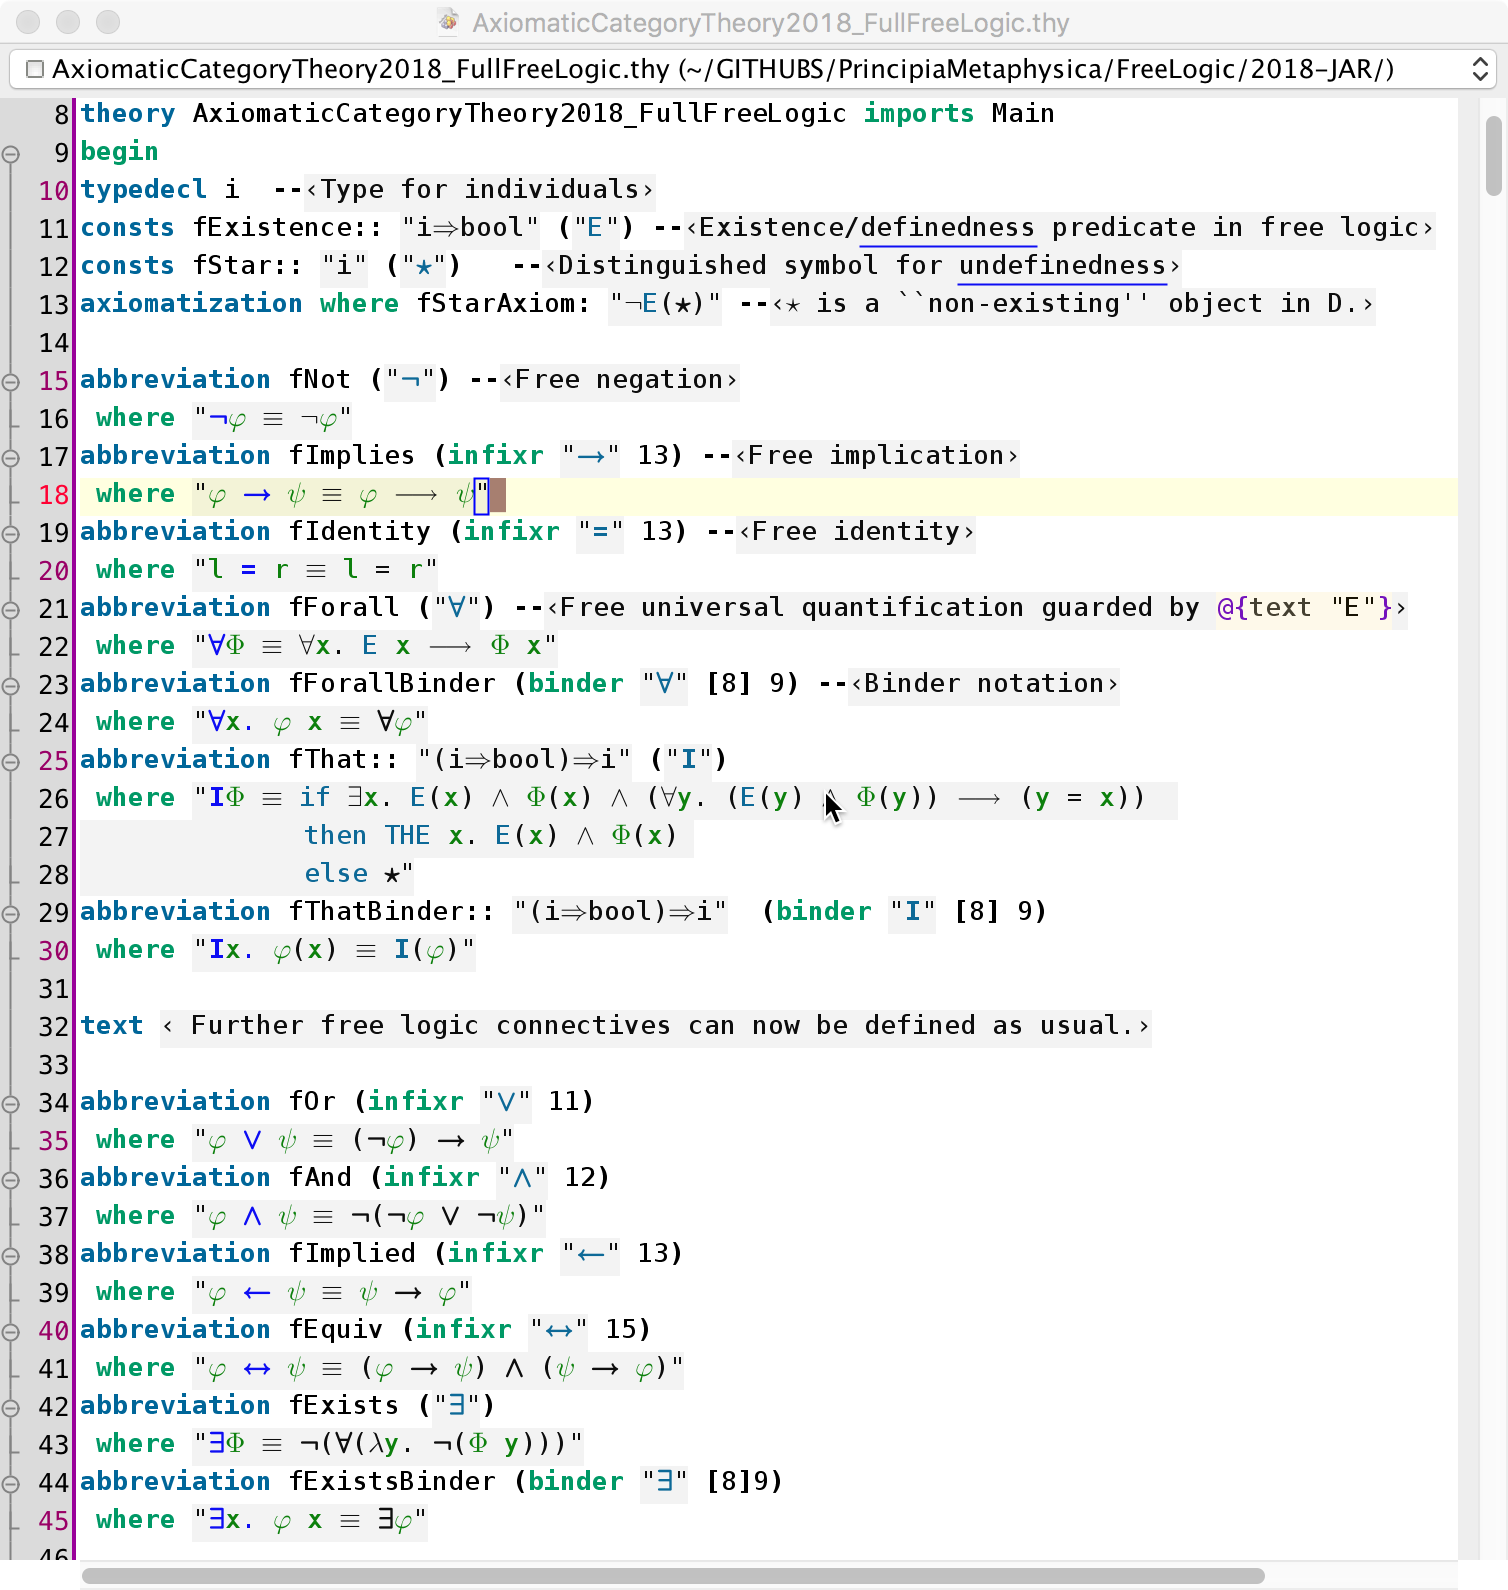
\includegraphics[width=\textwidth]{FFOL-Pic1}
 \caption{Isabelle/HOL encoding of $\FFOL$ (with $\star$ and definite description). \label{pic1}}
\end{figure}

\begin{figure}[htp]
 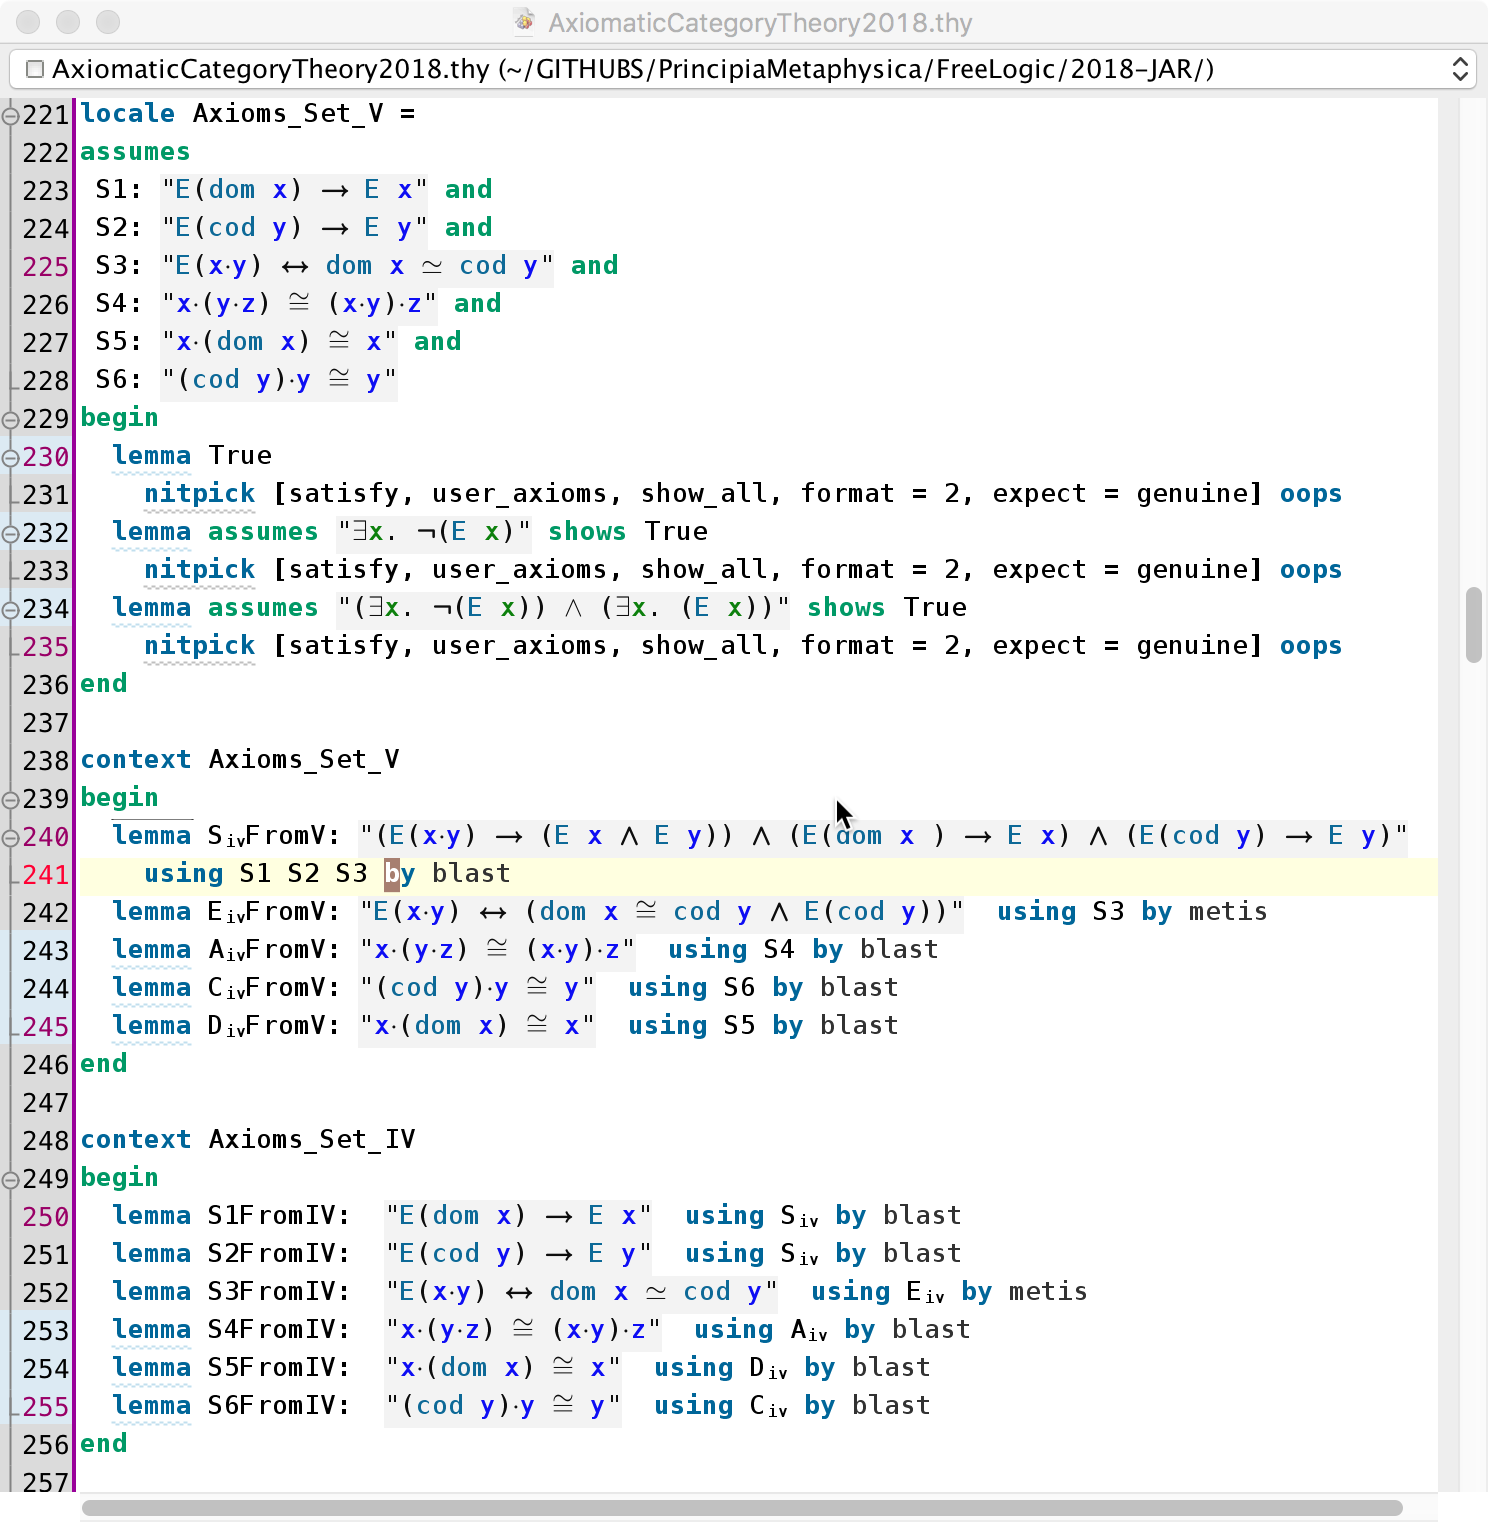
\includegraphics[width=\textwidth]{FFOL-Pic2}
 \caption{Encoding of Axioms Set V in Isabelle/HOL utilizing the
   embedded logic $\FFOL$; Axioms Set V is proven equivalent to Axioms
   Set IV. \label{pic2}}
\end{figure}




\begin{table}[htp] \centering \normalsize
\begin{tabular}{ll}
\hline
\\[-.8em]
\multicolumn{2}{c}{Axioms Set I} \\
%\hline
\\
 $S_{i}$ & $\ex(x \comp y) \imp (\ex x \wedge \ex y)$ \\
 $E_{i}$ & $\ex(x \comp y) \limp (\ex x \wedge \ex y \wedge (\exists z\lambdot z \comp
         z \cong z \wedge x \comp z \cong x \wedge z \comp y \cong y))$ \\
 $A_{i}$ & $x\comp (y \comp z) \cong (x \comp y) \comp z$ \\
 $C_{i}$ & $\forall y\lambdot \exists i\lambdot  \id i \wedge i \comp y \cong y$ \\
 $D_{i}$ & $\forall x\lambdot \exists j\lambdot  \id j \wedge x \comp j \cong x$  \\
\\
\hline
\\[-.8em]
\multicolumn{2}{c}{Axioms Set II} \\
%\hline
\\
$S_{ii}$ & $\ex(x \comp y) \imp (\ex x \wedge \ex y) \wedge (\ex (\dom x) \imp \ex
        x) \wedge (\ex (\cod y) \imp \ex
        y)$ \\
 $E_{ii}$ & $\ex(x \comp y) \limp (\ex x \wedge \ex y \wedge (\exists z\lambdot z \comp
         z \cong z \wedge x \comp z \cong x \wedge z \comp y \cong y))$ \\
 $A_{ii}$ & $x\comp (y \comp z) \cong (x \comp y) \comp z$ \\
 $C_{ii}$ & $\ex y \imp (\id(\cod y) \wedge (\cod y) \comp y \cong y)$ \\
 $D_{ii}$ & $\ex x \imp (\id(\dom x) \wedge x \comp (\dom x) \cong x)$ \\
\\
\hline
\\[-.8em]
\multicolumn{2}{c}{Axioms Set III} \\
%\hline
\\
$S_{iii}$ & $\ex(x \comp y) \imp (\ex x \wedge \ex y) \wedge (\ex (\dom x) \imp \ex
        x) \wedge (\ex (\cod y) \imp \ex
        y)$ \\
 $E_{iii}$ & $\ex(x \comp y) \limp (\dom x \cong \cod y \wedge \ex (\cod y)))$ \\
 $A_{iii}$ & $x\comp (y \comp z) \cong (x \comp y) \comp z$ \\
 $C_{iii}$ & $\ex y \imp (\id(\cod y) \wedge (\cod y) \comp y \cong y)$ \\
 $D_{iii}$ & $\ex x \imp (\id(\dom x) \wedge x \comp (\dom x) \cong x)$ \\
\\
\hline
\\[-.8em]
\multicolumn{2}{c}{Axioms Set IV} \\
%\hline
\\
$S_{iv}$ & $\ex(x \comp y) \imp (\ex x \wedge \ex y) \wedge (\ex (\dom x) \imp \ex
        x) \wedge (\ex (\cod y) \imp \ex
        y)$ \\
 $E_{iv}$ & $\ex(x \comp y) \biimp (\dom x \cong \cod y \wedge \ex (\cod y)))$ \\
 $A_{iv}$ & $x\comp (y \comp z) \cong (x \comp y) \comp z$ \\
 $C_{iv}$ & $(\cod y) \comp y \cong y$ \\
 $D_{iv}$ & $x \comp (\dom x) \cong x$  \\
\\
\hline
\\[-.8em]
\multicolumn{2}{c}{Axioms Set V (Scott 79, \cite{Scott79})} \\
%\hline
\\
$S1$ & $\ex (\dom x) \imp \ex x$ \\
$S2$ & $\ex (\cod y) \imp \ex y$ \\
$S3$ & $\ex(x \comp y) \biimp \dom x \simeq \cod y$ \\
$S4$ & $x\comp (y \comp z) \cong (x \comp y) \comp z$ \\
$S5$ & $(\cod y) \comp y \cong y$ \\
$S6$ & $x \comp (\dom x) \cong x$  \\
\\
\hline
\end{tabular}
\caption{Stepwise evolution of Scott's \cite{Scott79} axiom
  system for category theory from partial monoids. The axiom names are
  motivated as follows: 
  $S$ stands for strictness, $E$ for existence, $A$ for associativity, $C$ for
  codomain, $D$ for Domain. The free variables $x$, $y$, $z$ range over
  the raw domain $D$. The quantifiers in Axioms Sets I and II are
  free logic quantifiers, that is, they range over the domain $E$ of
  existing objects. \label{axioms-sets-1}}
\end{table}





\subsection{Modeling of basic concepts}
Morphisms in the category are modeled as objects in $D$ (respectively,
$\hol{D_i}$). We introduce three partial functions, 
$dom$ (domain), $cod$ (codomain), and $\comp$ (morphism composition). 
Partiality of composition is handled exactly as expected: we generally may have 
non-existing compositions $x\comp y$ (i.e. $\neg(\ex(x\comp y))$) for some existing  
morphisms $x$ and $y$ (i.e. $\ex x$ and $\ex y$).

For composition $\comp$ we assume set-theoretical composition here (i.e., functional 
composition from right to left). This means that
\[(\cod x) \comp (x \comp (\dom x)) \kleq x\] 
and that 
\[(x \comp y)a \kleq x(y a) \quad \text{when}\quad
\dom x \exid \cod y\] 
The equality symbol $\kleq$ denotes Kleene equality and it
is defined as follows (where $=$ is identity on all objects, existing or non-existing, 
of type $\ti$):
\[x \kleq y \ddef (\ex x \vee \ex y) \imp x = y\]
Existing identity $\simeq$ is defined as:
\[x \simeq y \ddef \ex x \wedge \ex y \wedge  x = y\]

$\cong$ is an equivalence relation. $\simeq$, in contrast, is only symmetric and transitive, and lacks 
reflexivity. These observations are quickly confirmed by Sledgehammer
in Isabelle.


Next, we define the identity morphism predicate $\id$ as follows: 

\[\id i \ddef (\forall x\lambdot \ex(i \comp x) \imp i \comp
x \cong x) \wedge (\forall x\lambdot \ex(x \comp i) \imp x \comp i \cong x)\]

This definition was suggested by an exercise in the textbook by Freyd
and Scedrov \cite{FreydScedrov90}
on p.~4.  In earlier experiments we used a longer definition which can
be proved equivalent on the basis of the other axioms. For monoids,
where composition is total, $\id i$ means $i$ is a two-sided identity
--- and such are unique. For categories the property is much weaker.
 

\subsection{Consistency}
The model finder Nitpick confirms consistency for all of the axioms
sets from Table~\ref{axioms-sets-1}. For example, when asked to consider at least one defined and one undefined object, then
Nitpick generates for all cases the following model (called $M_1$ in the remainder):
$D=\{i_i,i_2\}$ and $E=\{i_1\}$;  $i_1\comp i_1$ is $i_1$,  and $i_2$
in all other cases; $cod$ and $dom$ are identity on $D$. Without constraining the request, Nitpick
generates an even simpler model (called $M_0$ in the remainder):
$D=\{i_i\}$ and $E=\emptyset$; $i_1\comp i_1$ is $i_1$; $cod$ and
$dom$ are identity on $D$. It is trivial to check that these models
indeed confirm the consistency of all axioms sets from Table~\ref{axioms-sets-1}.

  % Constants:
   % codomain = (λx. _)(i⇩1 := i⇩1)
   %  op ⋅ = (λx. _)((i⇩1, i⇩1) := i⇩1)
   %  domain = (λx. _)(i⇩1 := i⇩1)
   %  E = (λx. _)(i⇩1 := False)


  % Constants:
  %   codomain = (λx. _)(i⇩1 := i⇩1, i⇩2 := i⇩2)
  %   op ⋅ = (λx. _)((i⇩1, i⇩1) := i⇩1, (i⇩1, i⇩2) := i⇩2, (i⇩2, i⇩1) := i⇩2, (i⇩2, i⇩2) := i⇩2)
  %   domain = (λx. _)(i⇩1 := i⇩1, i⇩2 := i⇩2)
  %   E = (λx. _)(i⇩1 := True, i⇩2 := False)



\subsection{Axioms Sets I and II}
 Axioms Set I is our most basic set of axioms for category theory generalizing the 
axioms for a monoid to a partial composition operation. Remember that a monoid is an 
algebraic structure $(S,\circ)$, where $\circ$ is a binary operator on set $S$, 
satisfying the following properties: 
$$
\begin{tabular}{ll}
Closure: & $ \forall a,b \in S\lambdot \ a \circ b \in S$ \\
Associativity: & $\forall a,b,c \in S\lambdot\ a \circ (b \circ c) = (a \circ b) \circ c$ \\
Identity: & $\exists id_S \in S\lambdot \forall a\in S\lambdot \ id_S\circ a = a = a \circ id_S$
\end{tabular}
$$

That is, a monoid is a semigroup with a two-sided identity element.

Axioms Set I generalizes the notion of a monoid by introducing a partial, strict binary 
composition operation $\comp$. The existence of left and right identity elements is 
addressed in the last two axioms. The notions of $dom$ (domain) and
$cod$ (codomain)
abstract from their common meaning in the context of sets. In category theory we
work with just a single type of objects (the type $\hol{i}$ in our setting) and therefore 
identity morphisms are employed to suitably characterize their
meanings.

We can prove that the $i$ in axiom $C_i$ and the $j$ in axiom $D_i$
are unique. The proofs and the dependencies can be 
   found automatically by Sledgehammer.
$$  \forall y\lambdot \exists i\lambdot \id i \wedge i \comp y \cong y
\wedge (\forall j\lambdot d(\id j \wedge j \comp y \cong y) \imp i \cong j)
\quad 
    (\text{by } A_i, C_i, S_i) $$
$$ \forall x\lambdot \exists j\lambdot \id j \wedge x \comp j \cong x \wedge
(\forall i\lambdot (\id i \wedge x \comp i \cong x) \imp j \cong i) \quad   
    (\text{by }  A_i, D_i, S_i) $$

However, the $i$ and $j$ need not be equal. Using existential
variables $C$ and $D$, this can be encoded in
   our formalization as follows: 
 $$\exists C\lambdot \exists D\lambdot (\forall y\lambdot \id (C y) \wedge (C y) \comp y \cong y)
 \wedge (\forall x\lambdot \id (D x) \wedge x \comp (D x) \cong x) \wedge
 D \not= C$$

The model finder Nitpick confirms that this formula is satisfiable:
e.g. choose domain $D=\{i_1,i_2\}$ and $E=\{i_2\}$; $i_2\comp i_2$ returns $i_2$,  and $i_1$
in all other cases; variable $D$ is identity on domain $D$, but $C$ maps both
$i_1$ and $i_2$ to $i_2$. 


%\subsection{Axioms Set II}
Axioms Set II is developed from Axioms Set I by Skolemization of the
existentially quantified variables $i$ and $j$ in axioms $C_i$ and
$D_i$. We can argue semantically that every model of Axioms Set I has
such functions. Hence, we get a conservative extension of Axioms Set
I. This could be done for any theory with an ``$\forall x\lambdot \exists i\lambdot$''-axiom. The strictness axiom $S$ is extended, so
that strictness is now also postulated for the new Skolem functions
$dom$ and $cod$. Note that the values of Skolem functions
outside $E$ can just be given by the identity function.

The left-to-right direction of existence axiom $E_{ii}$ is implied. 
  $$E(x \comp y) \imp (E x \wedge E y \wedge (\exists z\lambdot z \comp z
  \cong z \wedge x \comp z \cong x \wedge z\comp y \cong y)) \quad
  (\text{by } A_{ii}, C_{ii}, S_{ii})$$

Axioms $C_{ii}$ and $D_{ii}$, together with $S_{ii}$, show that
${\dom}$ and ${\cod}$ are total functions, as intended: 
$$E x \imp E(\dom x) \quad (\text{by } D_{ii}, S_{ii})$$
$$E x \imp E(\cod x) \quad (\text{by } C_{ii}, S_{ii}) $$

The proofs are found by the Sledgehammer tool and automatically
reconstructed in Isabelle/HOL. Further information on these
experiments are provided in \S\ref{sec-remarks-experiments}
below. Using Sledgehammer we have also shown that Axioms Set II
implies Axioms Set I. Vice versa, Axioms Set I also implies Axioms Set
II. This can easily be shown by semantical means on the meta-level.

\subsection{Remark on the Experiments}  \label{sec-remarks-experiments}
% \marginpar{Include remark on SMT calls and the SMT tactic (see Reviewer 1)}
% \marginpar{Include remark on Sledgehammer and how it works (see
%   Reviewer 1)}
% \marginpar{Add footnote on some issues with Sledgehammer, Z3 and Spass}

All proofs above and all proofs in the rest of this paper (unless
stated otherwise) have been obtained fully automatically in very
reasonable time (typically just a few seconds) with the
Sledgehammer tool in Isabelle/HOL (version Isabelle2017). This tool interfaces to prominent
first-order automated theorem provers such as CVC4 \cite{CVC4}, Z3
\cite{Z3}, E \cite{E} and Spass \cite{Spass}.  Remotely, also
  provers such as Vampire \cite{Vampire}, or the higher-order provers
  Satallax \cite{Satallax} and LEO-II \cite{LEO} can be reached. For
  example, to prove axiom $E_{iii}$ from Axioms Set II, we have called
  Sledgehammer on all axioms of Axioms Set II. The provers then, via
  Sledgehammer, suggested to call trusted/verified tools in
  Isabelle/HOL with the exactly required dependencies they
  detected, in this case $C_{ii}$, $D_{ii}$, $E_{ii}$ and $S_{ii}$. With the provided dependency information the trusted tools
  in Isabelle/HOL were then able to reconstruct the external proofs on
  their own.  This way we obtain a verification of our claims in
  Isabelle/HOL, in which all the proofs have nevertheless been
  contributed by automated theorem provers. For further information on
  the use and functioning of Sledgehammer we refer to the 
  literature \cite{Sledgehammer,SledgehammerTutorial}.

  In our experiments we have also made use of the Isabelle/HOL's
  \textsc{smt} method, which ``translates the conjecture and any
  user-supplied facts to the SMT solvers’ many-sorted first-order
  logic, invokes a solver, and (depending on the solver) either trusts
  the result or attempts to reconstruct the proof in Isabelle.''
  \cite[p.~5]{Sledgehammer}.\footnote{Technical remark: We have
    selected CVC4 in our experiments as the default SMT solver, since
    we did run into errors when working with Z3. These errors can
    easily be reconstructed in the provided source files when
    switching back to Z3 as default.}  For quite some time the use of
  the \textsc{smt} method has been controversially discussed in the
  Isabelle/HOL community, and there is in fact a significant difference
  between using the \textsc{smt} method in combination with Z3 or with
  CVC4, as we prefer. When setting the solver to CVC4, the contributed
  proofs are accepted and being trusted without replaying them in the
  Isabelle kernel. Proofs contributed by Z3, in contrast, are never
  trusted and always replayed in Isabelle's kernel. For the work
  presented here this community internal discussion is of minor
  relevance, so that we decided to continue working with CVC4 in order
  to keep our formalisation concise and also because CVC4
  performed surprisingly well in our experiments.\footnote{An expert
    reviewer of this article, to whom we are very grateful, provided
    alternative proofs which can be
    fully replayed in the kernel of Isabelle.}

% \marginpar{Remove this part? SMT is now called as an oracle.}
%   However, there are still
%   a few calls of the \textsc{smt}-tactic contained in our document, 
%    which we found are not entirely trivial to replace. In this sense, our
%    Isabelle/HOL verification is modulo the correctness of the \textsc{smt} solvers
%    CVC4 \cite{CVC4} and Z3 \cite{Z3}.





\subsection{Axioms Sets III, IV and V} 
In Axioms Set III the existence  axiom  $E_{ii}$ from Axioms Set II  is simplified by taking advantage of 
  the two new Skolem functions ${\dom}$ and $cod$.

The left-to-right direction of existence axiom $E_{iii}$ is implied.
  $$E(x \comp y) \imp (\dom x \cong \cod y \wedge E(\cod y)) \quad  
    (\text{by } A_{iii}, C_{iii}, D_{iii}, S_{iii})$$

 % Axioms Set II and Axioms Set III are equivalent; this has been
 % confirmed by the automated theorem provers and verified in Isabelle/HOL.

%\subsection{Axioms Set IV}
Axioms Set IV simplifies the axioms $C_{iii}$ and  $D_{iii}$. However, as it turned 
 out, these simplifications also require the existence axiom $E_{iii}$ to be strengthened into
 an equivalence.

 % Axioms Set III and Axioms Set IV are equivalent; this has been
 % confirmed by the automated theorem provers and verified in
 % Isabelle/HOL.

%\subsection{Axioms Set V}
Axioms Set V has been proposed by Scott \cite{Scott79} in the 1970s. 
This set of axioms is equivalent to the axioms set presented by Freyd
and Scedrov in their textbook ``Categories, Allegories''
\cite{FreydScedrov90}, when encoded in free logic, corrected/adapted
and further simplified.  Their axioms set is technically flawed when
encoded in our given context. This issue has been detected by
automated theorem provers with the same technical infrastructure as
employed so far. See \S\ref{sec-freyd-scedrov} for more
details. 

 Axioms Sets II, III, IV and V are equivalent; this has been
 automatically 
 confirmed by the automated theorem provers and verified in
 Isabelle/HOL.

 \section{Assessment of the Axiom System by Freyd and
   Scedrov} \label{sec-freyd-scedrov} In this section we study the
 axioms set of Freyd and Scedrov from their textbook ``Categories,
 Allegories'' \cite{FreydScedrov90}.  In \S\ref{subsec-freyd-scedrov-1} we show that their axioms set,
 replicated in Table~\ref{axioms-sets-2} as Axioms Set FS-I, becomes
 inconsistent in our free logic setting if we assume non-existing
 objects in $D$, respectively, if we assume that the operations
 are non-total.


\begin{table} \centering \normalsize
\begin{tabular}{ll}
\hline
\\
\multicolumn{2}{c}{Axioms Set FS-I:  Freyd and Scedrov in original notation (with issues)} \\
%\hline
\\
  $A1$ &  $\ex(x \circ y) \longleftrightarrow (x\Box \cong \Box y)$ \\ 
  $A2a$ & $((\Box x)\Box) \cong \Box x$ \\ 
  $A2b$ & $\Box (x\Box) \cong \Box x$ \\ 
  $A3a$ & $(\Box x) \circ x \cong x$ \\ 
  $A3b$ & $x \circ (x\Box) \cong x$ \\ 
  $A4a$ & $\Box(x \circ y) \cong \Box(x \circ (\Box y))$ \\ 
  $A4b$ & $(x \circ y)\Box \cong ((x\Box) \circ y)\Box$ \\ 
  $A5$   & $x \circ (y \circ z) \cong  (x \circ y) \circ z$ \\
\\
\hline
\\
\multicolumn{2}{c}{Axioms Set FS-II: Freyd and Scedrov in our notation (with issues)} \\
%\hline
\\
  $A1$  & $\ex (x \comp y) \longleftrightarrow \dom x \cong \cod y$ \\
  $A2a$ & $\cod(\dom x) \cong \dom x$ \\  
  $A2b$ & $\dom(\cod y) \cong \cod y$ \\  
  $A3a$  & $x \comp (\dom x) \cong x$ \\ 
  $A3b$ & $(\cod y) \comp y \cong y$ \\
  $A4a$ & $\dom(x \comp y) \cong \dom((\dom x) \comp y)$ \\ 
  $A4b$ & $\cod(x \comp y) \cong \cod(x \comp (\cod y))$ \\ 
  $A5$   & $x \comp (y \comp z) \cong  (x \comp y) \comp z$   \\
\\
\hline
\\
\multicolumn{2}{c}{Axioms Set VI: Freyd and Scedrov in our notation
(corrected)} \\
%\hline
\\
  $A1'$  & $\ex (x \comp y) \longleftrightarrow \dom x \simeq\cod y$ \\
  $A2a$ & $\cod(\dom x) \cong \dom x$ \\  
  $A2b$ & $\dom(\cod y) \cong \cod y$ \\  
  $A3a$  & $x \comp (\dom x) \cong x$ \\ 
  $A3b$ & $(\cod y) \comp y \cong y$ \\
  $A4a$ & $\dom(x \comp y) \cong \dom((\dom x) \comp y)$ \\ 
  $A4b$ & $\cod(x \comp y) \cong \cod(x \comp (\cod y))$ \\ 
  $A5$   & $x \comp (y \comp z) \cong  (x \comp y) \comp z$   \\
\\
\hline
\end{tabular}
\caption{The axioms set of Freyd and Scedrov in their and our
  notation, together with a proposed correction.\label{axioms-sets-2}}
\end{table}


 Note, however, that the free variables in this first study range over
 the existing and non-existing objects in $D$. One may argue,
 that this is not the intention of Freyd and
 Scedrov. Therefore, we add a second study in \S\ref{subsec-freyd-scedrov-2}, in which we restrict the
 variables to range only over existing objects in $E$. However, also in this case
 the axiom system of Freyd and Scedrov remains unsatisfactory. Now it
 turns out incomplete, 
 since strictness conditions/axioms are required which are not mentioned in
 the textbook.

  Freyd and Scedrov employ a different notation for $\dom x$ and $\cod
 x$. They denote these operations by $\Box x$ 
  and $x\Box$. Moreover, they employ diagrammatic composition $(f \circ
  g) x \cong g(f x)$ (functional composition from left to right) instead of the set-theoretic 
  definition $(f \comp g) x \cong f(g x)$ (functional composition from right to left) used so far.
  We leave it to the reader to verify that their Axioms
  Set FS-I corresponds to Axioms
  Set FS-II modulo an appropriate conversion of notation.\footnote{A recipe for 
  this translation is as follows: (i) replace all $x \circ y$ by
  $y \comp x$, (ii) rename the variables to get them again in alphabetical order,
(iii) replace $\varphi\Box$ by $\cod \varphi$ and $\Box\varphi$  by $\dom \varphi$, and finally
(iv) replace $\cod y \cong \dom x$ (resp. $\cod y \simeq \dom x$) 
   by $\dom x \cong \cod y$ (resp. $\dom x \simeq \cod y$).}

 \subsection{Constricted Inconsistency in Free Logic
   Setting} \label{subsec-freyd-scedrov-1} A main difference in the
 system by Freyd and Scedrov to our Axioms Set V from Table~\ref{axioms-sets-1} concerns axiom $S3$, respectively $A1$. Namely,
 instead of the non-reflexive existing identity $\simeq$, they use
 Kleene equality $\cong$, cf. definition 1.11 on page 3 of their textbook
 \cite{FreydScedrov90}.\footnote{Def. 1.11 in Freyd Scedrov: ``The
   ordinary equality sign $=$ [i.e., our $\cong$] will be used in the
   symmetric sense, to wit: if either side is defined then so is the
   other and they are equal. \ldots''} The difference seems minor, but
 in our free logic setting it has the effect to cause the mentioned
 constricted inconsistency issue.\footnote{This could perhaps be an
   oversight, or it could indicate that Freyd and Scedrov actually
   mean the Axioms Set discussed in \S\ref{subsec-freyd-scedrov-2}
   below.%  (where the variables in the axioms range over defined objects
   % only). However, in this reading of the axioms of Freyd and Scedrov
   % we had to (re-)introduce explicit strictness conditions to ensure
   % equivalence to the Axioms Set V by Scott.
 }

  The (constricted) inconsistency of Axioms Set FS-I, respectively
  Axioms Set FS-II, from Table~\ref{axioms-sets-2} has been 
  detected first by the model finder Nitpick. When we asked Nitpick to
  generate a model with at least one non-existing object, it claimed
  that there is no such model. However, a model can still be
  constructed if we do not make any assumptions about non-existing
  objects.\footnote{For this we have to inactivate the axiom
    that postulates that $\star$ is an undefined/non-existing object.} In fact, the model presented by Nitpick for this case
  consists of a single, existing morphism.

However, one can see directly that Axiom $A1$ is problematic
as written: If $x$ and $y$ are undefined, then
(presumably) $\dom x$ and $\cod y$ are undefined as
well, and by the definition of Kleene equality, $\dom x \cong \cod
  y$. $A1$ stipulates that $x \comp y$ should be defined in
this case, which appears unintended.

As we will demonstrate now, the consequences of this version of the axiom are
even stronger. It implies that \emph{all} objects are defined,
that is, composition (as well as $dom$ and $cod$) become total operations.
The theory described by these axioms ``collapses'' to the theory of
monoids: If all objects are defined, then one can conclude from $A1$ that 
$\dom x \cong \dom y$ (resp.~$\dom x \cong \cod y$) and $\cod x \cong \cod y$), 
and according to 1.14 of \cite{FreydScedrov90}, 
the category reduces to a monoid provided that it is not empty.

In fact, the automated theorem provers, via Sledgehammer, quickly
prove falsity from Axioms Sets FS-II and FS-I when assuming a 
 non-existing object of type $\hol{i}$:
$$(\exists x\lambdot \neg E x) \imp False$$

The provers identify the axioms $A1$,
 $A2a$ and $A3a$ to cause the problem under this assumption. A
 corresponding  human-intuitive proof argument is as follows:
 
 Let $a\in D$ be an undefined object, that is, assume $\neg E a$.  By
 instantiating axiom $A3a$ with $a$ we have $a \comp (\dom a) \cong a$.  From
 this and definition of $\cong$ we know that $a \comp (\dom a)$ is not
 defined. This is easy to see, since if $a \comp (\dom a)$ were defined, we
 also had that $a$ is defined, which is not the case by assumption.
  Hence, $\neg E (a \comp (\dom a)$.
Next, we instantiate $A1$ with $a$ and $\dom a$ to obtain
   $E(a \comp (\dom a)) \biimp \dom a \cong \cod(\dom a)$. Moreover,
   by instantiating $A2a$ with $a$ we obtain $\cod(\dom a) \cong \dom a$,
   which we use (modulo symmetry and transitivity of $\cong$) to
   rewrite the former result into 
   $E(a \comp (\dom a)) \biimp \dom a \cong \dom a$. By reflexivity of
   $\cong$ we thus get $E(a \comp (\dom a))$, i.e. that $a \comp
   (\dom a)$ is defined, which contradicts $\neg E (a \comp (\dom
   a)$. $\Box$

As a corollary from the above constricted inconsistency result we get
that all morphisms (objects in $D$) must be
defined: $\forall x\lambdot E x$.




% We also
%  show
%  that there is a simple fix to that issue, namely to replacement of
%  the occurence of Kleene equality in one axiom by  

% We have modified the axioms of \cite{FreydScedrov90} by
% replacing the original Kleene equality $\cong$ in their axiom $S3$ by
% the non-reflexive, existing identity $\simeq$. Note that the modified
% axiom $S3$ is equivalent to $E_{iv}$.\marginpar{Check again} 

%  this study we assume 

% However, this time we restrict 
% the free variables in their system to range over existing objects only. By employing the free logic 
% universal quantifier @{text "❙∀"} we thus modify Axiom Set VII as follows:


\begin{table} \centering \normalsize
\begin{tabular}{ll}
\\
\hline
\\
\multicolumn{2}{c}{Freyd and Scedrov in our notation (corrected and
  reduced I)} \\
%\hline
\\
  $A1'$  & $\ex (x \comp y) \longleftrightarrow \dom x \simeq\cod y$ \\
  $A3a$  & $x \comp (\dom x) \cong x$ \\ 
  $A3b$ & $(\cod y) \comp y \cong y$ \\
  $A4a$ & $\dom(x \comp y) \cong \dom((\dom x) \comp y)$ \\ 
  $A4b$ & $\cod(x \comp y) \cong \cod(x \comp (\cod y))$ \\ 
  $A5$   & $x \comp (y \comp z) \cong  (x \comp y) \comp z$   \\
\\
\hline
\\
\multicolumn{2}{c}{Freyd and Scedrov in our notation (corrected and
  reduced II)} \\
%\hline
\\
  $A1'$  & $\ex (x \comp y) \longleftrightarrow \dom x \simeq\cod y$ \\
  $A2a$ & $\cod(\dom x) \cong \dom x$ \\  
  $A2b$ & $\dom(\cod y) \cong \cod y$ \\  
  $A3a$  & $x \comp (\dom x) \cong x$ \\ 
  $A3b$ & $(\cod y) \comp y \cong y$ \\
  $A5$   & $x \comp (y \comp z) \cong  (x \comp y) \comp z$   \\
\\
\hline
\\
\multicolumn{2}{c}{Freyd and Scedrov in our notation (corrected and
  reduced III)} \\
%\hline
\\
 $S^1_{v}$ & $\ex (\dom x) \imp \ex x$ \\
  $S^2_{v}$ & $\ex (\cod y) \imp \ex y$ \\
  $A1'$  & $\ex (x \comp y) \longleftrightarrow \dom x \simeq\cod y$ \\
  $A3a$  & $x \comp (\dom x) \cong x$ \\ 
  $A3b$ & $(\cod y) \comp y \cong y$ \\
  $A5$   & $x \comp (y \comp z) \cong  (x \comp y) \comp z$   \\
\\
\hline
\end{tabular}
\caption{Reduced variants of Axioms Set VI.\label{axioms-sets-3}}
\end{table}

Obviously Axioms Sets FS-I and FS-II are also redundant, and we have previously reported 
on respective redundancies \cite{ICMS}.\footnote{The discussion in our releated
  conference paper \cite{ICMS} was before the discovery of the above 
constricted inconsistency issue, which tells us that the system (in our setting) can even be reduced 
to axioms A1, A2a, and A3a (when we assume undefined objects).} For
the corrected Axioms Set VI we still get redundancies. The different options to reduce this system are reported in
Table~\ref{axioms-sets-3}.

Attempts to remove axioms A1', A3a, A3b, and A5 from Axiom Set VI failed. Nitpick shows that they are independent. 

However, when assuming strictness of $dom$ and $\cod$, the axioms
A2a, A2b, A4a and A4b are all implied. Hence, under this 
   assumptions, the reasoning tools quickly identify (A1' A3a A3b A5) as a minimal axiom 
   set, which then exactly matches the Axioms Set V of Scott from Table~\ref{axioms-sets-1}.\footnote{This minimal set of axioms 
   has also been mentioned by Freyd in a note \cite{Freyd16} and attributed to Martin Knopman. However, the proof
   sketch presented there seems to fail when the adapted version of A1 (with $\simeq$) is employed.}



\begin{table} \centering \normalsize
\begin{tabular}{ll}
\hline
\\
\multicolumn{2}{c}{Axioms Set FS-III: Freyd and Scedrov in our notation (with issues)} \\
%\hline
\\
  $B1$  & $\all{x}\all{y} \ex (x \comp y) \longleftrightarrow \dom x \cong \cod y$ \\
  $B2a$ & $\all{x} \cod(\dom x) \cong \dom x$ \\  
  $B2b$ & $\all{y} \dom(\cod y) \cong \cod y$ \\  
  $B3a$  & $\all{x} x \comp (\dom x) \cong x$ \\ 
  $B3b$ & $\all{y} (\cod y) \comp y \cong y$ \\
  $B4a$ & $\all{x}\all{y} \dom(x \comp y) \cong \dom((\dom x) \comp y)$ \\ 
  $B4b$ & $\all{x}\all{y} \cod(x \comp y) \cong \cod(x \comp (\cod y))$ \\ 
  $B5$   & $\all{x}\all{y}\all{z} x \comp (y \comp z) \cong  (x \comp y) \comp z$   \\
\\
\hline
\\
\multicolumn{2}{c}{Axioms Set FS-IV: Freyd and Scedrov in our
  notation (without issues)} \\
%\hline
\\
 $B0a$ & $\ex (x \comp y) \longrightarrow  (\ex x \wedge \ex y)$ \\
 $B0b$ & $\ex (\dom x)  \longrightarrow   \ex x$ \\
 $B0b$ & $\ex (\cod x)  \longrightarrow   \ex x$ \\
  $B1$  & $\all{x}\all{y} \ex (x \comp y) \longleftrightarrow \dom x \cong \cod y$ \\
  $B2a$ & $\all{x} \cod(\dom x) \cong \dom x$ \\  
  $B2b$ & $\all{y} \dom(\cod y) \cong \cod y$ \\  
  $B3a$  & $\all{x} x \comp (\dom x) \cong x$ \\ 
  $B3b$ & $\all{y} (\cod y) \comp y \cong y$ \\
  $B4a$ & $\all{x}\all{y} \dom(x \comp y) \cong \dom((\dom x) \comp y)$ \\ 
  $B4b$ & $\all{x}\all{y} \cod(x \comp y) \cong \cod(x \comp (\cod y))$ \\ 
  $B5$   & $\all{x}\all{y}\all{z} x \comp (y \comp z) \cong  (x \comp y) \comp z$   \\
\\
\hline
\end{tabular}
\caption{The axioms set of Freyd and Scedrov in our
  notation and with variable restriction to existing objects only.\label{axioms-sets-4}}
\end{table}

\subsection{Missing Strictness Axioms in Alternative
  Setting} \label{subsec-freyd-scedrov-2} We study the axiom system by
Freyd and Scedrov once again. However, this time we restrict the free
variables in their system to range over existing objects only. In the
context of algebraic theories, it could be argued that this is the
preferred reading of free variables.  By employing the free logic
universal quantifier $\forall$, which realizes such a restriction, 
we thus modify Axioms Set FS-II into
Axioms-Set FS-III as displayed in Table~\ref{axioms-sets-4}.  

For Axioms Set FS-III the consistency checks with Nitpick succeed,
even if we assume undefined objects. However, this axioms set is
obviously weaker than Axioms Set V from Table~\ref{axioms-sets-1}. In fact, as has been shown by Nitpick, none of
the axioms of this set are implied.  The situation changes when we
explicitly postulate strictness of $dom$, $cod$ and $\comp$. Doing
so we obtain Axioms Set FS-IV from Table~\ref{axioms-sets-4}, which,
as Nitpick confirms, is consistent even if we assume undefined
objects. And the automated theorem provers via Sledgehammer confirm
that Axioms Set FS-IV is equivalent to Axioms Set V, as
intended. Unfortunately, however, respective strictness conditions are
not mentioned in the textbook by Freyd and Scedrov.





\section{Summary and Further Work}
We have developed a new reasoning framework for free logic, and we
have experimentally applied it for some first experiments in category
theory.  We have demonstrated how modern proof assistants and theorem
provers for classical higher-order logic may well support the
reasoning in free logic. More concretely, we have applied our new free
logic reasoning framework for the systematic exploration of axiom
systems for category theory. Without tools, support of such experiments
would be extremely tedious and error prone.
In the course of our experiments, automated theorem provers 
have revealed some (minor) issue in the textbook of Freyd and Scedrov \cite{FreydScedrov90},
which we were able to correct. The correction essentially corresponds
to the axiom system by Scott proposed earlier \cite{Scott67}.
All our findings were achieved directly by or in
close interaction with automated reasoning tools. 
Perhaps the lesson to be learned here is that, when working with partial functions,
it is natural --- out of caution  --- to assume too much, and the automated reasoning
tools, as we have shown here, can help find in what ways the axioms might be reduced or
simplified.

% % Our free logic reasoning framework is publicly available for reuse:
% Simply download Isabelle from https://isabelle.in.tum.de and
% initialize it (respec- tively import) the file FreeFOL.thy from our
% sources available at
% www. christoph-benzmueller.de/papers/2016-ICMS.zip. Our category
% theory experiments are contained in the file FreydScedrov.thy.


Comparisons with other theorem provers for free logic are not possible at this stage, since we are not aware of any other existing systems.

Further work includes the extension of our work towards an embedding
of free higher-order logic, the continuation of our formalization
studies in category theory (especially extensions of the theory
involving functors) and the application of free logic to
various other mathematical domains, including, for example, projective
geometry.  Regarding extensions towards free higher-order logic some
first steps have already been taken
\cite{W56,makarenko16:_autom_logik_logik_stufe}, and a recent
continuation of our formalisation studies \cite{J39} now also includes 
an early axiom system for category theory by Saunders MacLane
\cite{maclane48:_group}.


Moreover, as an alternative to always unfolding the mapping from
$\FFOL$ to $\HOL$, abstract level proof tactics could be provided
e.g. in Isabelle/HOL to support intuitive interaction (and even
automation) in $\FFOL$ on top the semantical embedding.

\begin{acknowledgements}
 We thank G{\"u}nter Rote, Lutz Schr\"oder and and Emil Weydert for their
comments to \cite{ArXiv}, which together with \cite{ICMS} forms the
basis for this article.

We also want to express our gratitude to the reviewers of this
article.  Their fruitful feedback definitely helped to improve the
final version.
\end{acknowledgements}

% BibTeX users please use one of
%\bibliographystyle{spbasic}      % basic style, author-year citations
\bibliographystyle{spmpsci}      % mathematics and physical sciences
%\bibliographystyle{spphys}       % APS-like style for physics
\bibliography{bibliography}   % name your BibTeX data base

% % Non-BibTeX users please use
% \begin{thebibliography}{}
% %
% % and use \bibitem to create references. Consult the Instructions
% % for authors for reference list style.
% %
% \bibitem{RefJ}
% % Format for Journal Reference
% Author, Article title, Journal, Volume, page numbers (year)
% % Format for books
% \bibitem{RefB}
% Author, Book title, page numbers. Publisher, place (year)
% % etc
% \end{thebibliography}

\end{document}
% end of file template.tex

